\documentclass{article}

\usepackage[T1]{fontenc}
\usepackage{amsmath}
\usepackage{amssymb}
\usepackage{graphicx}
\usepackage{titling}
\usepackage{ragged2e}
\usepackage{lipsum}
\usepackage{booktabs}
\usepackage{fancyvrb}
\usepackage[hidelinks]{hyperref}
\usepackage[a4paper,left=0.75in,right=0.75in,top=1in,bottom=1in,footskip=0.5in]{geometry}

\pretitle{\vspace{1in}\hrulefill\par}
\posttitle{\par\hrulefill}

\title{\begin{center}\Huge COMP2432\\
    G06 Group Project Reoprt\end{center}}
\date{}
\author{}

\begin{document}
    \begin{titlepage}
        \maketitle
        \begin{center}
            \huge Room Booking Manager
            \vfill
            \begin{table}[!htbp]
                \centering
                \huge
                \begin{tabular}{ll}
                    19081789D\hspace{0.25in}&MAN, Furui \\
                    19078543D\hspace{0.25in}&WANG, Meng \\
                    18080998D\hspace{0.25in}&WU, Junyu  \\
                    19079008D\hspace{0.25in}&XING, Shiji\\
                \end{tabular}
            \end{table}
            \vspace{0.5in}
            \thispagestyle{empty}
        \end{center}
    \end{titlepage}
    \cleardoublepage
    \tableofcontents
    \thispagestyle{empty}
    \cleardoublepage
    \setcounter{page}{1}
    \section{Introdoction}
        \paragraph{}
        The project aims to utilize the knowledge covered in COMP2432 Operating Systems
        and put them into practice to get a further understanding and improvement. 
        This work is based on the scenario of implementing of a room booking manager
        for a frictional company, PolySME Bussiness center. By making advantage of
        various abstracted skills covered in the lecture , i.e. scheduling algorithms,
        multi-process programming, and interprocess communication a simple scheduler
        core and related utilities is developed.
    \cleardoublepage
    \section{Scope}
        \subsection{Multi-Process Programming and Inter-process Communication}
            \paragraph{}
            Scheduling module is implemented as a child process created via fork(). The communication between parent and scheduling module is based on pipe(), write(), and read(). In addition, in order to deliver complex information, we use pointers and pipes together. To utilize CPU, child processes are created for different scheduling methods, so that they can run at same time. The parent process uses read() and write() to synchronize among childern and to control the order of output. Additionally, since opti works on the basis of prio scheduling, the result of prio scheduling is directly passed to opti via mother process in order to avoid redundant computations.
        \subsection{ CPU Scheduling}
            \paragraph{}
            In this project, we are required to implement FCFS and prio algorithm for component booking, which is similar to what we learned in lectures about CPU Scheduling. However, there are some difference between algorithms in CPU scheduling and booking scheduling. In booking scheduling, we only care about the order of coming request and don't mind exact arrival time. In CPU scheduling, processes can be finished while in booking scheduling, requests can't be finished during the scheduling. Thus, the method to implement booking scheduling algorithms is similar to but still differs from CPU scheduling.
        \subsection{Memory Allocation}
            \paragraph{}
            Thinking of rooms as fixed partitions and requests as jobs, the process of allocating rooms for requests has the same logic as Multi-programming with a Fixed number of Tasks, where we have fixed amount of resources which is divided into certain numbers of partitions, and our task is to allocate different amounts of resources for objects in need of resources.
        \subsection{Synchronization}
            \paragraph{}
            Program-Monitored Synchronization is used for development. Since three children are running scheduling algorithms independently, some measure must be taken to synchronize and control the output. The parent process uses pipes to send signals to childs to control their behaviors, so that they can perform the scheduling algorithms simultaneously and be able to print results in order.
    \cleardoublepage
    \section{Concept}
        \subsection{FCFS Scheduling}
            \paragraph{}
                First-Come-First-Serve(aka, FCFS) handles requests upon a first-come-first-serve basis. Later requests that cause collision are rejected, otherwise are accepted.
            \paragraph{}
                In its implementation, no sorting is needed because the order of the request link-list during scheduling is exactly the same as that of input, given that the invalid ones have been filtered out. The only thing to note is that to maintain the order of requests, Input-Handler Module must be single-threaded.
            \paragraph{}
                Below is a illustration of FCFS algorithm. Green-colored requests are accepted, whereas red-colored requests are rejected, and the requests arrive in sequence indicated by arrows between. 
            \begin{figure}[!htbp]
                \centering
                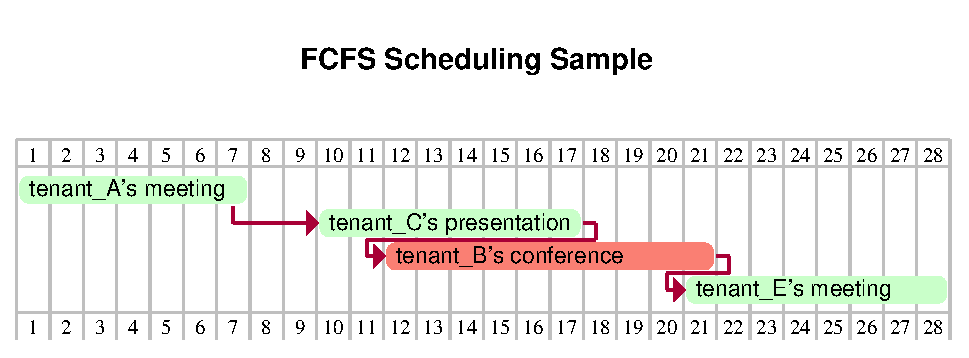
\includegraphics[scale=0.7]{eps/fcfs_scheduling.eps}
                \caption{Gantt Diagram for FCFS algorithm Sample output for one single Room}
            \end{figure}
        \subsection{PRIO Scheduling}
            \paragraph{}
            Priority scheduling(aka, PRIO) is the scheduling algorithm based on the
                priority of requests. Rather than that in FCFS which indicated by arriving time, the priority are implied within the requests weighted by its type (i.e. device-booking, meeting, presentation, or conference). 
            \paragraph{}
            To implement PRIO, the tasks required is to stably sort the request link-list upon user-defined priority, then call FCFS scheduling. This would reuse the code and decrease the overall complexity of the program.
                Requests are stored in an array after sortion based on priority. 
            \paragraph{}
            Below is the visualization of PRIO scheduling, with the same annotation rules as used in FCFS.
            \begin{figure}[!htbp]
                \centering
                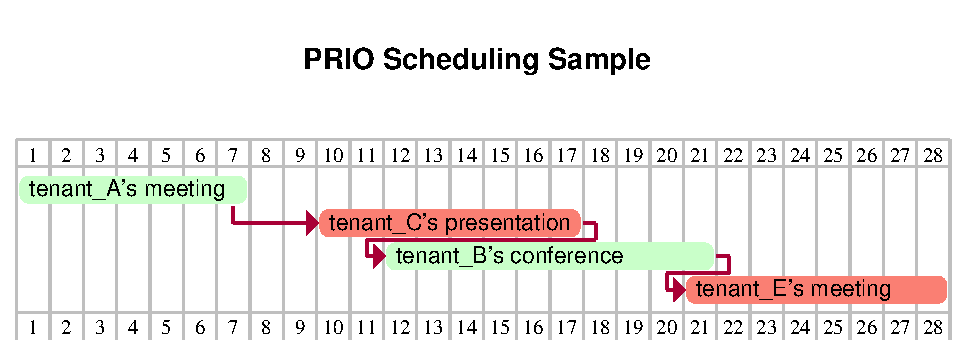
\includegraphics[scale=0.7]{eps/prio_scheduling.eps}
                \caption{Gantt Diagram for PRIO algorithm Sample output for one single Room}
            \end{figure}
        \subsection{OPTI Scheduling}
            \paragraph{}
                Optimized Scheduling bases on the result of PRIO or FCFS scheduling and it rescheduled the valid failed requests. The process first finds a desired time slot  of a rejected request, and try to "push" this time slot to both sides until it finds a suitable time slot for this request. Then it selects one that is closer to the original desired time slot and update the request. The process repeats this procedure untill all requests that can be rescheduled is rearranged.
    \cleardoublepage
    \section{Algorithm}
    \subsection{Design of own algorithm}
        \paragraph{Optimization Algorithm}
        \paragraph{}
            Optimization algorithm is based on processed result by FCFS algorithm or
            PRIO algorithm. Failed requests from the two algorithm firstly undergo
            verification. Valid requests are rescheduled based on bi-directional
            search of linked lists of rooms and devices. 

    \cleardoublepage

    \section{Program Structure}
        \subsection{Class Design}
            \begin{figure}[!htbp]
                \centering
                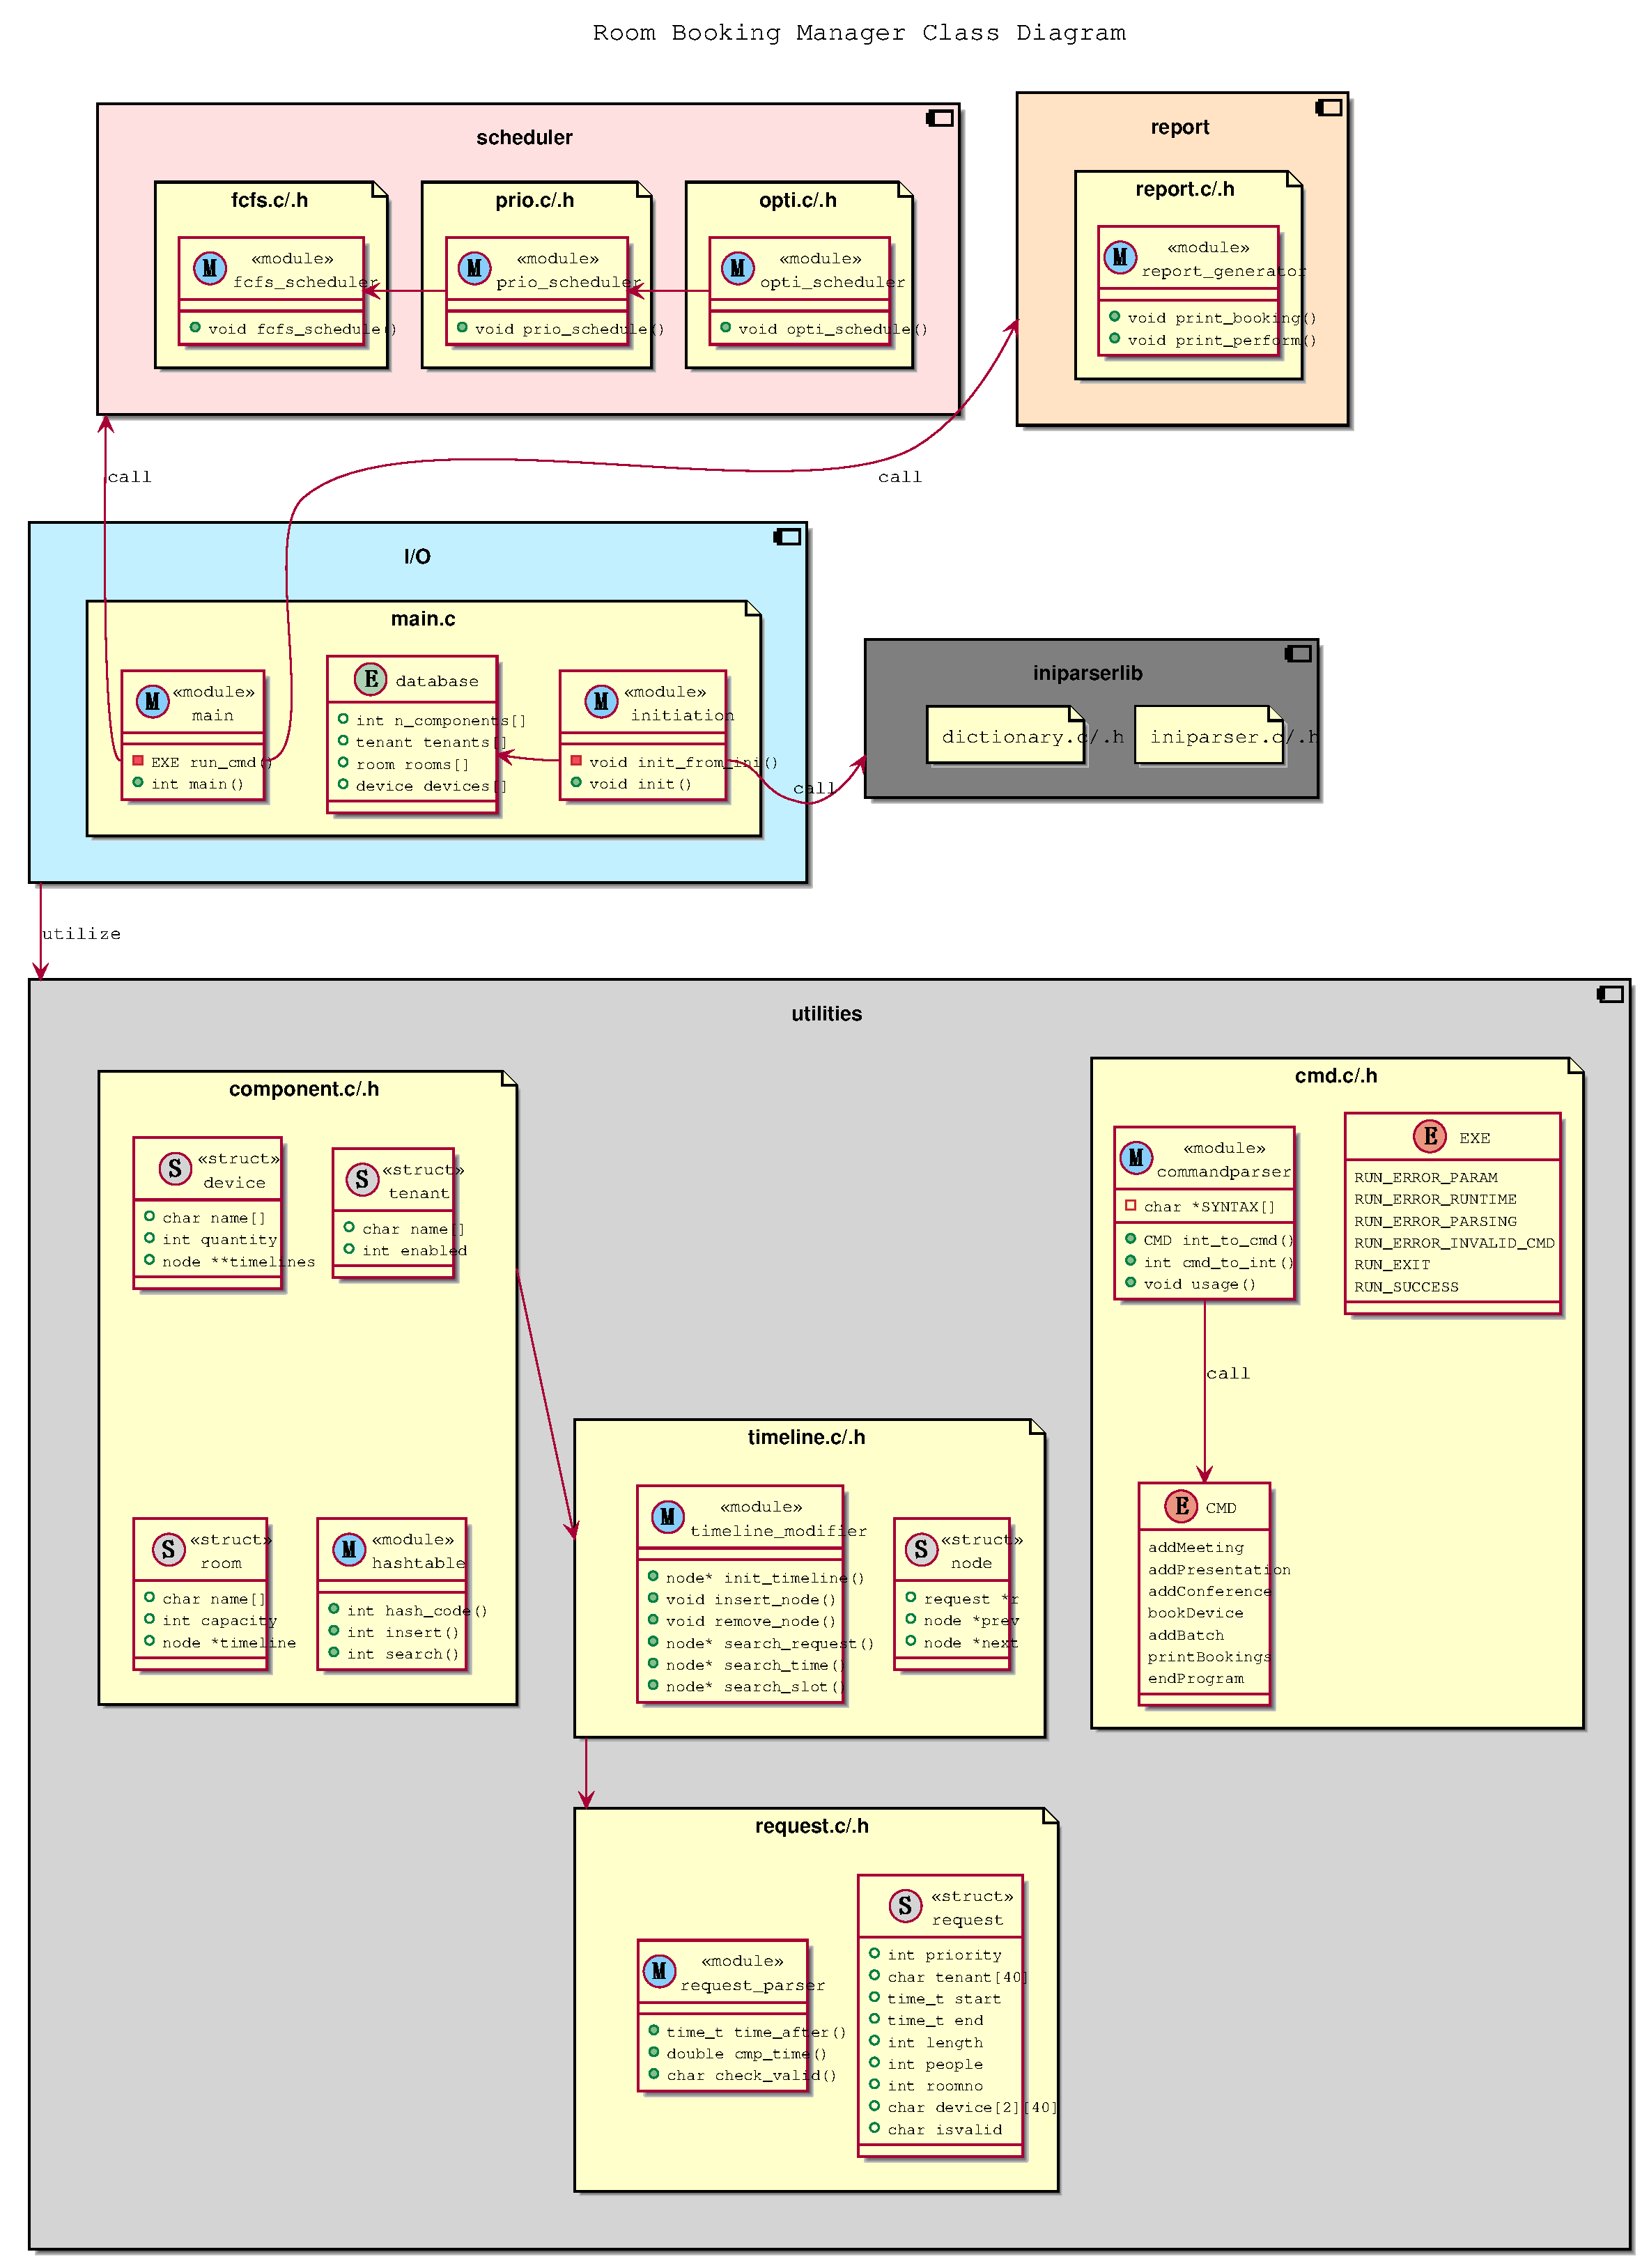
\includegraphics[scale=0.4]{eps/class_diagram.eps}
                \caption{Overall class design diagram of Room Booking Manager}
            \end{figure}
        \subsection{Activity Design}
            \begin{figure}[!htbp]
                \centering
                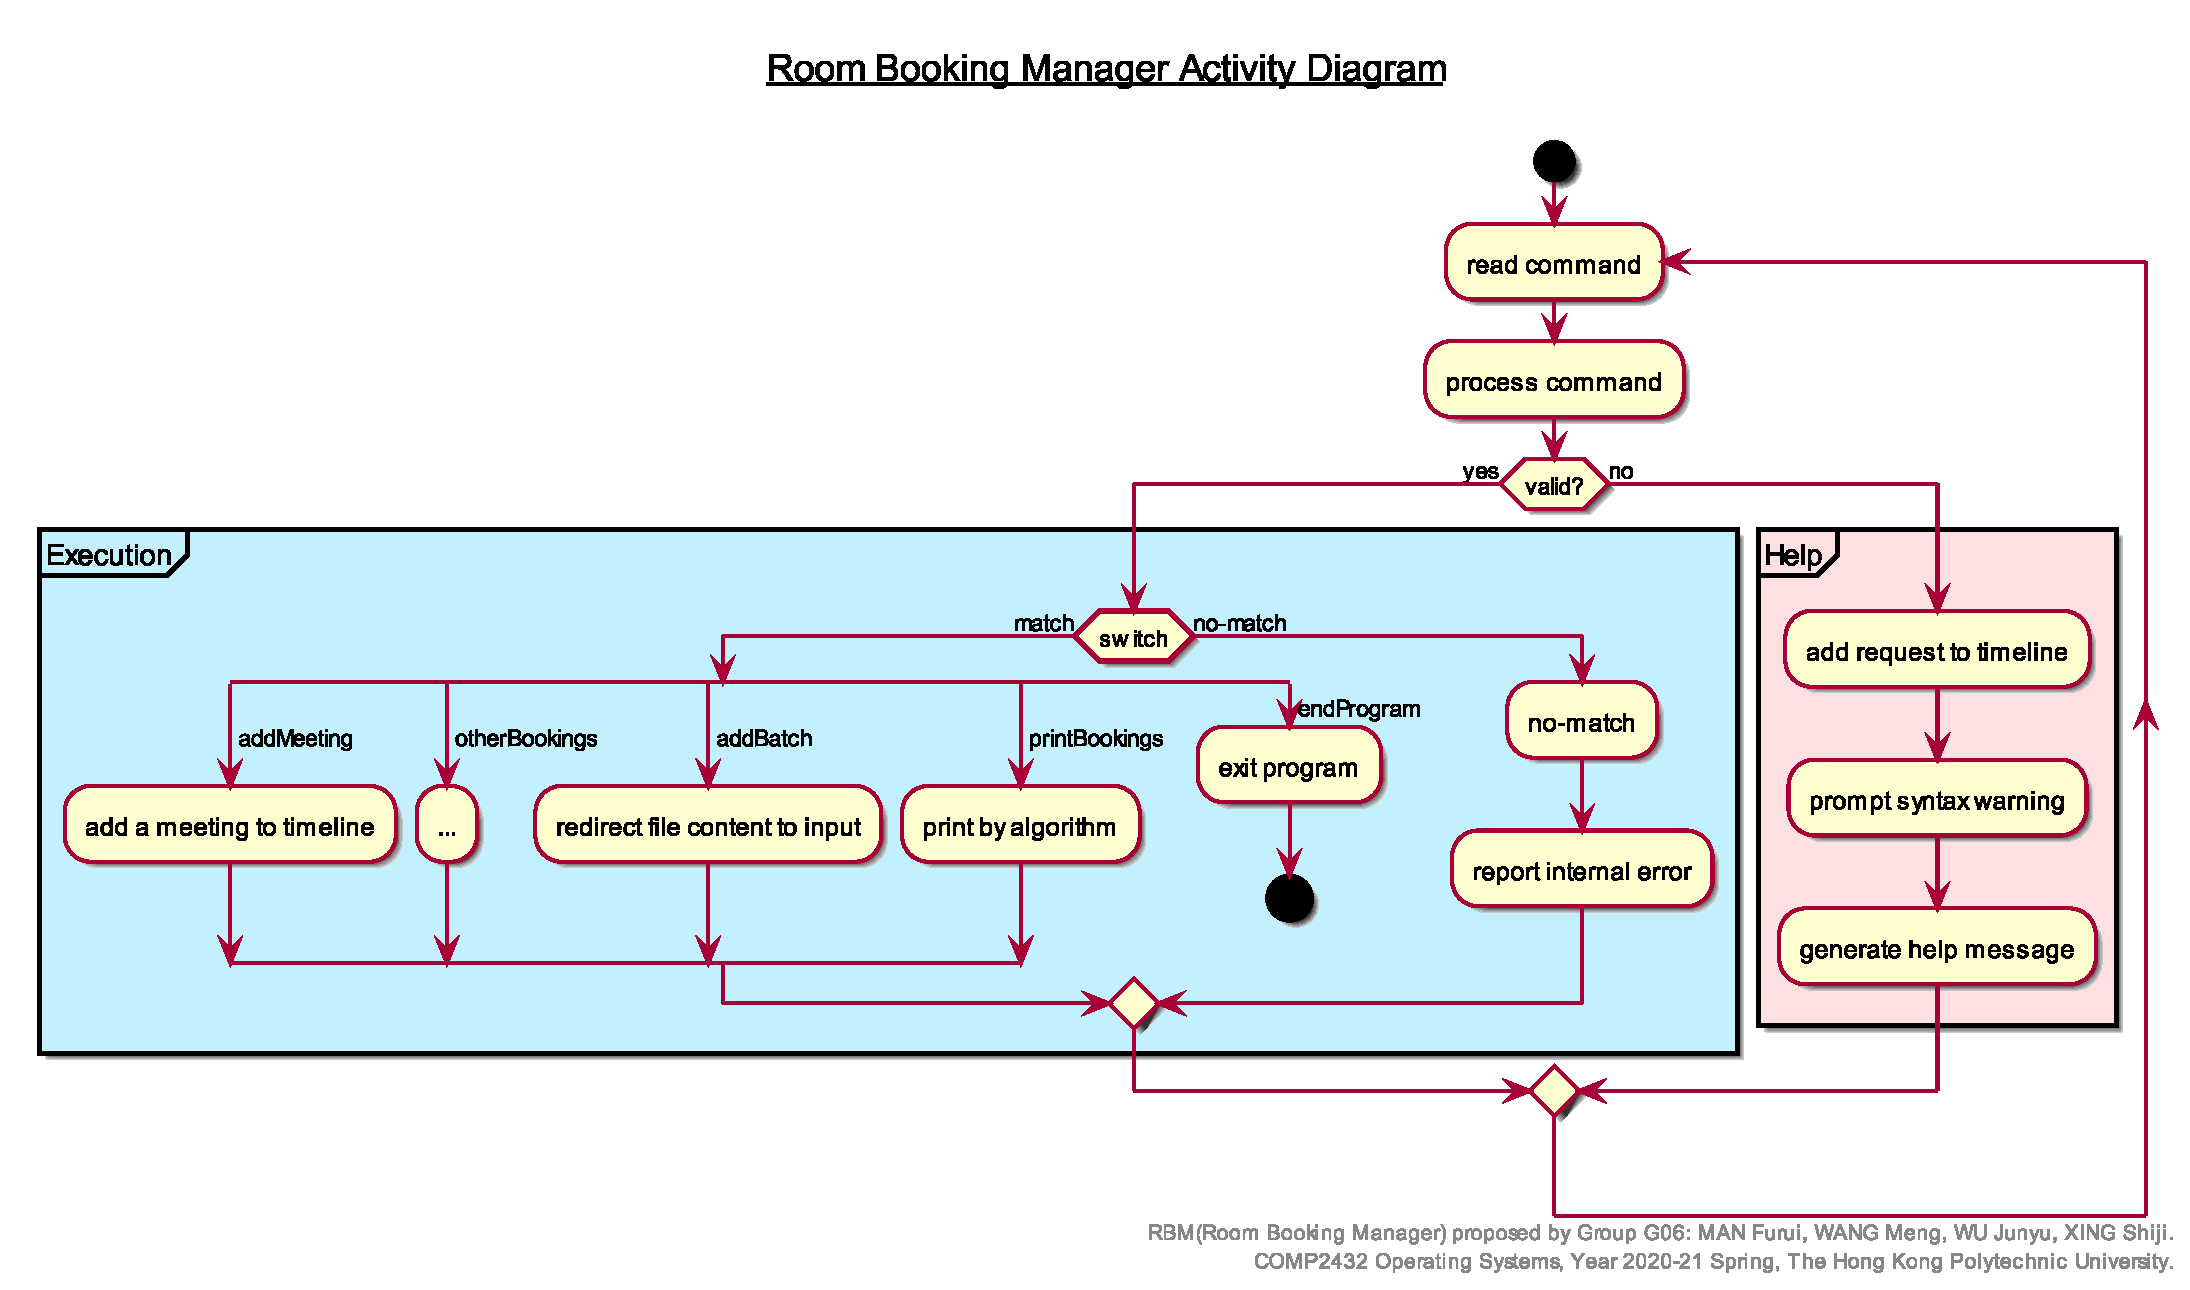
\includegraphics[scale=0.45]{eps/activity_diagram.eps}
                \caption{Overall activity design diagram of Room Booking Manager}
            \end{figure}
    \cleardoublepage
    \section{Testing Cases}
        \paragraph{}
        This is the brief version, which demonstrates the valid and invalid tests for \texttt{addMeeting} instruction only.
        \paragraph{}
        Tests for other instructions are similar and therefore not included. Syntax of other instructions varies in
        number of the parameters. Help message on syntax is available once an input error is detected.
        \paragraph{}
        Refer to the appendix for the full version. 

        \subsection{Valid Tests}
            \paragraph{}
            Valid syntax for \texttt{addMeeting} instruction should be:
            \begin{Verbatim}[gobble=8]
                addMeeting -tenant YYYY-MM-DD hh:mm n.n [d1 d2]; 
            \end{Verbatim}
            \paragraph{}
            Below are some samples which conforms the above syntax:
            \begin{Verbatim}[gobble=8]
                addMeeting -tenant_A 2021-05-10 21:50 1.5 5 projector_2K screen_100;
                addMeeting -tenant_A 2021-05-11 18:20 0.3 5;
                addMeeting -tenant_A 2021-05-11 04:10 0.1 5;
            \end{Verbatim}
        
        
        \subsection{Invalid Tests}
            \paragraph{}
            Invalid instructions of addMeeting contains either:
            
            \begin{itemize}
            \item Syntax invalid: (including command invalid, tenant invalid, date invalid, hour and minute invalid,
            duration invalid, number of people invalid, device invalid); or
            \end{itemize}
            
            \begin{Verbatim}[gobble=8]
                command_invalid and parameters does not matter;
                addMeeting -tenant_invalid 2021-05-10 1:30 0.5 5 projector_2K screen_100;
                addMeeting -tenant_A date-in-valid 1:30 0.5 5 projector_2K screen_100;
                addMeeting -tenant_B 2021-05-10 hhmm:invalid 1.5 5 webcam_FHD monitor_75;
                addMeeting -tenant_C 2021-05-10 18:30 duration.invalid 5 webcam_FHD monitor_50;
                addMeeting -tenant_D 2021-05-10 10:40 0.1 peopleinvalid projector_2K screen_150;
                addMeeting -tenant_D 2021-05-16 3:10 1.1 5 device_invalid monitor_50;
            \end{Verbatim}
            \begin{itemize}
            \item Device pairing error (devices must be in pairs).
            \end{itemize}
            \begin{Verbatim}[gobble=8]
                addMeeting -tenant_E 2021-05-10 22:20 0.5 5 projector_4K monitor_50; 
                addMeeting -tenant_E 2021-05-10 22:20 0.5 5 projector_4K; 
            \end{Verbatim}
        

    \cleardoublepage
    \section{Performance analysis}
    \paragraph{}
        The utilization of FCFS and prio are similar to each other and whose utilization is higher depends on the data given since the we can get the output of prio by giving FCFS the reordered input data of prio. However, in most cases, the performance of prio is better than FCFS. Because prio guarantee that more important bookings are severed while the utilization is not lowwer in general.  
    \paragraph{}
        Based on the result of FCFS and prio, opti improves the utilization while guaranteeing more important bookings are served. If we don't take into account that sometimes it is very unfair to users who come first (now their bookings may be canceled only because some later bookings with the same priority takes longer time), the performance of opti is the best.
    \paragraph{}
        In conclusion, opti has the best performance in our opinion, because it maintains a relatively good balance between efficiency and fairness.
    \cleardoublepage
    \section{Program Setup \& Analysis}
        \subsection{Program Setup}
            \paragraph{Step 0 Clone repo (optional)}
            \paragraph{}
                Clone the repo from Github if there is no local copy.
            \begin{Verbatim}[gobble=8]
                git clone https://github.com/toolsmax0/COMP2432_RBM.git
            \end{Verbatim}
            \paragraph{Step 1 Compilation}
            \paragraph{}
                \texttt{cd} to the project's root directory and execute \texttt{build.sh} script.
            \paragraph{}
                The program have dependency upon \texttt{gcc 4.0+} and \texttt{linux 3.0+}.
            \begin{Verbatim}[gobble=8]
                cd COMP2432_RBM
                sh build.sh
            \end{Verbatim}
            \paragraph{Step 2 Customization (optional)}
            \paragraph{}
                To modify the component settings (i.e. tenants, rooms, devices),
                modify \texttt{RBM.ini} file according to its syntax.
            \paragraph{Step 3 Execution}
            \paragraph{}
                To execute the program, run the following command.
            \begin{Verbatim}[gobble=8]
                ./out/RBM
            \end{Verbatim}

        \subsection{Progarm Analysis}
            
    \cleardoublepage
    \section{Appendix}
        \subsection{Source Code}
            \paragraph{}
                All source files are located under \texttt{./src/} directory. Please \texttt{cd}
                to corresponding directory for reference.
            \paragraph{}
                Content of \texttt{main.c} is shown below
            \begin{Verbatim}[gobble=8]
                #include "master.h"
                #include <unistd.h>
                #include <sys/wait.h>
                #include <stdio.h>
                #include <stdlib.h>
                #include <stdint.h>
                
                // #define _DEBUG
                
                // collection of num_tenants, num_rooms, num_devices
                int n_components[3];
                tenant tenants[1000];
                
                room rooms[1000];
                device devices[1000];
                int devices_t[1000];
                int home[1000];
                const int PRIME = 997;
                request requests[10000];
                FILE *IStreams[100];
                int isi = 0;
                time_t genesis;
                time_t eternity;
                int requestno;
                
                void schedule(int);
                int openBatch(char *s);
                /**
                 * @brief initiate all available devices from RBM.ini
                 */
                int init_from_ini()
                {
                #define INIT(val, f, s)                                 \
                    int n_##s = iniparser_getsecnkeys(d, #s);           \
                    const char *name_##s[n_##s];                        \
                    iniparser_getseckeys(d, #s, name_##s);              \
                    for (int i = 0; i < n_##s; i++)                     \
                    {                                                   \
                        sscanf(name_##s[i], #s ":%s", val[i].name);     \
                        val[i].f = iniparser_getint(d, name_##s[i], 0); \
                    }
                #define _INIT_DEBUG(val, f, s)                      \
                    printf("No. of " #s " available: %d\n", n_##s); \
                    for (int i = 0; i < n_##s; i++)                 \
                        printf("  %d: %s @%d\n", i, val[i].name, val[i].f);
                
                    dictionary *d = iniparser_load("RBM.ini");
                    INIT(devices, quantity, devices);
                    INIT(rooms, capacity, rooms);
                    INIT(tenants, enabled, tenants);
                
                    n_components[0] = n_tenants,
                    n_components[1] = n_rooms,
                    n_components[2] = n_devices;
                
                #ifdef _DEBUG
                    _INIT_DEBUG(devices, quantity, devices);
                    _INIT_DEBUG(rooms, capacity, rooms);
                    _INIT_DEBUG(tenants, enabled, tenants);
                #endif
                
                    return 0;
                }
                
                /**
                 * @brief run a single cmd, returns execution status
                 * 
                 * @param   cmd     short command type in int, see enum CMD
                 * @param   param   parameters for the command
                 * @return  execution status in int, see enum EXE in lib/cmd.h
                 */
                EXE run_cmd(int cmd, char *param, request *rq, int *newreq)
                {
                    // printf("accepted: \"%s\", ", param);
                    int n_param, duration[2];
                    struct tm s; // start time
                
                #define HANDLE_PARAM_ERR \
                    if (!rq->isvalid)    \
                        return RUN_ERROR_PARAM;
                #define SCAN_PARAM_FOR_ADD_FUNCTIONS(rq, s, len)                                        \
                    n_param = sscanf(                                                                   \
                        param, "-%s %d-%d-%d %d:%d %d.%d %d %s %s",                                     \
                        rq->tenant, &(s.tm_year), &(s.tm_mon), &(s.tm_mday), &(s.tm_hour), &(s.tm_min), \
                        &len[0], &len[1], &rq->people, rq->device[0], rq->device[1]);
                
                #define SCAN_PARAM_POSTPROCESS(rq, s, len)           \
                    s.tm_year -= 1900;                               \
                    s.tm_mon -= 1;                                   \
                    s.tm_sec = 0;                                    \
                    rq->start = mktime(&s);                          \
                    rq->end = time_after(rq->start, len[0], 6 * len[1]); \
                    rq->roomno = -1;                                 \
                    rq->length = 60 * len[0] + 60 * 0.1 * len[1];
                
                    switch (cmd)
                    {
                    case addMeeting:
                        *newreq = 1;
                        SCAN_PARAM_FOR_ADD_FUNCTIONS(rq, s, duration)
                        rq->priority = 2;
                        rq->isvalid = (n_param == 11) || (n_param == 9);
                        SCAN_PARAM_POSTPROCESS(rq, s, duration)
                        rq->isvalid &= check_valid(rq);
                
                        HANDLE_PARAM_ERR
                        // addMeeting executions
                        puts("executing addMeeting");
                        break;
                
                    case addPresentation:
                        *newreq = 1;
                        SCAN_PARAM_FOR_ADD_FUNCTIONS(rq, s, duration)
                        rq->priority = 1;
                        rq->isvalid = (n_param == 11);
                        SCAN_PARAM_POSTPROCESS(rq, s, duration)
                        rq->isvalid &= check_valid(rq);
                
                        HANDLE_PARAM_ERR
                        // addPresentation executions
                        puts("executing addPresentation");
                        break;
                
                    case addConference:
                        *newreq = 1;
                        SCAN_PARAM_FOR_ADD_FUNCTIONS(rq, s, duration)
                        rq->priority = 0;
                        rq->isvalid = (n_param == 11);
                        SCAN_PARAM_POSTPROCESS(rq, s, duration)
                        rq->isvalid &= check_valid(rq);
                
                        HANDLE_PARAM_ERR
                        // addConference executions
                        puts("executing addConference");
                        break;
                
                    case bookDevice:
                        *newreq = 1;
                        n_param = sscanf(
                            param, "-%s %d-%d-%d %d:%d %d.%d %s",
                            rq->tenant, &s.tm_year, &s.tm_mon, &s.tm_mday, &s.tm_hour, &s.tm_min,
                            &duration[0], &duration[1], rq->device[0]);
                        rq->device[1][0] = 0;
                        rq->isvalid = (n_param == 9);
                        rq->priority = 3;
                        rq->people = 0;
                        SCAN_PARAM_POSTPROCESS(rq, s, duration)
                        rq->isvalid &= check_valid(rq);
                
                        HANDLE_PARAM_ERR
                        // bookDevice executions
                        puts("executing bookDevice");
                        break;
                
                    case addBatch:;
                
                        char filename[40];
                        n_param = sscanf(param, "-%s", filename);
                        if (n_param != 1)
                            return RUN_ERROR_PARAM;
                        // the above also affects the following return status RUN_ERROR_PARAM
                        puts("executing addBatch");
                        return openBatch(filename);
                        break;
                
                    case printBookings:;
                        char algo[20];
                        sscanf(param, "-%s", algo);
                        int type = 0;
                        switch (algo[0])
                        {
                        case 'f':
                            if (strcmp(algo, "fcfs"))
                                return RUN_ERROR_PARAM;
                            type = 1;
                            break;
                        case 'p':
                            if (strcmp(algo, "prio"))
                                return RUN_ERROR_PARAM;
                            type = 2;
                            break;
                        case 'o':
                            if (strcmp(algo, "opti"))
                                return RUN_ERROR_PARAM;
                            type = 3;
                            break;
                        case 'A':
                            if (strcmp(algo, "ALL\0"))
                                return RUN_ERROR_PARAM;
                            type = 4;
                            break;
                        default:
                            return RUN_ERROR_PARAM;
                        }
                        schedule(type);
                        break;
                
                    case endProgram:
                        return RUN_EXIT;
                    case INVALID:
                        return RUN_ERROR_INVALID_CMD;
                    // cmd (string) -> (int) parsing error!
                    default:
                        return RUN_ERROR_PARSING;
                    }
                    return RUN_SUCCESS;
                }
                
                void init()
                {
                    init_from_ini();
                    struct tm genesis_s = {0, 0, 0, 1, 0, 0};
                    struct tm eternity_s = {0, 0, 0, 1, 0, 130};
                    genesis = mktime(&genesis_s);
                    eternity = mktime(&eternity_s);
                    IStreams[0] = stdin;
                    memset(devices_t, -1, sizeof(devices_t));
                    for (int i = 0; devices[i].name[0] != 0; i++)
                    {
                        insert(i);
                        node **timelines=calloc(devices[i].quantity,sizeof(node*));
                        for (int j = 0; j < devices[i].quantity; j++)
                            timelines[j] = init_timeline();
                        devices[i].timelines = timelines;
                    };
                    for (int i = 0; rooms[i].name[0] != 0; i++)
                    {
                        rooms[i].timeline = init_timeline();
                    }
                }
                
                int main()
                {
                    init();
                    // struct tm tmp = {tm_year : 2021-1900, tm_mon : 4-1, tm_mday : 1};
                    // time_t t1 = mktime(&tmp);
                    // time_t t2 = time_after(t1, 2, 0);
                    // request tmp0 = {1, "tenant_a", t1, t2, 120, 5,isvalid:1};
                    // request tmp1 = {0, "test tenant2", t1, t2, 120, 15, 0, "webcam_fhd", "screen_150",isvalid:1};
                    // request tmp2 = {3, "device", t1, t2, 120, 0, 0, "webcam_fhd", "screen_150",isvalid:1};
                    // request *test[] = {&tmp0, &tmp1, &tmp2,0};
                    // request *success[1000]={};
                    // request *fail[1000]={};
                    // fcfs_schedule(test, success, fail);
                    // print_booking(success,fail,"FCFS");
                    // print_perform(success,fail,"FCFS");
                    // opti_schedule(test, success, fail);
                    // schedule(4);
                    // return 0;
                
                    int cmd_int, execution;
                    char input[MAX_INPUT_LENGTH];
                    char cmd[MAX_CMD_LENGTH], param[MAX_PARAM_LENGTH];
                    do
                    {
                        printf("RBM# ");
                        char st[1000] = {};
                        char check[100] = {};
                        fgets(st, 200, stdin);
                        if (sscanf(st, "%[^;]%s", input, check) == EOF)
                        {
                            if (!isi)
                            {
                                puts("ERROR: No more commands to be read, exiting.");
                                return -1;
                            }
                            fclose(IStreams[isi--]);
                            stdin = IStreams[isi];
                            continue;
                        }
                        if (*check != ';')
                        {
                            puts("Syntax Error: Missing Semi-Column, Skipping.");
                        }
                        sscanf(input, "%s %[^;]", cmd, param);
                        cmd_int = cmd_to_int(cmd);
                        int newreq = 0;
                        // < 0 then error occured
                        if ((execution = run_cmd(cmd_int, param, requests + requestno, &newreq)) < RUN_EXIT)
                        {
                            switch (execution)
                            {
                            case RUN_ERROR_PARAM:
                            case RUN_ERROR_INVALID_CMD:
                                // intended, two cases with same handling
                                usage(cmd_int);
                                break;
                            case RUN_ERROR_RUNTIME:
                            case RUN_ERROR_PARSING:
                                puts("this is a bug");
                                break;
                
                            default:
                                puts("Error detected.");
                                break;
                            }
                        }
                        if (newreq)
                            requestno++;
                #ifdef _DEBUG
                        printf("----DEBUG: cmd @%d, cmd|parm @%s|%s, execution @%d\n", cmd_int, cmd, param, execution);
                #endif
                    } while (execution != RUN_EXIT);
                
                    printf("quit loop, exiting main program\n");
                }
                
                int cmp(const void *x, const void *y)
                {
                    request *a = *(request **)x;
                    request *b = *(request **)y;
                    return a->priority - b->priority;
                }
                
                int cmp2(const void *x, const void *y)
                {
                    request *a = *(request **)x;
                    request *b = *(request **)y;
                    int first = strcmp(a->tenant, b->tenant);
                    if (first)
                        return first;
                    return cmp_time(a->start, b->start);
                }
                int cmp3(const void *x, const void *y)
                {
                    request *a = *(request **)x;
                    request *b = *(request **)y;
                    return cmp_time(a->start, b->start);
                }
                /**
                 * Inter-Process signal:
                 *  Parent to Child:
                 *      1:fcfs scheduling;
                 *      2:prio scheduling;
                 *      3:opti scheduling;
                 *      4:opti scheduling with preprocessed data;
                 *      5:print scheduling result;
                 *      6:print scheduling analysis;
                 *      7:fetch preprocessed data
                 *      8:exit;
                 *  Child to Parent:
                 *      1: current job finished;
                 **/
                void schedule(int algo)
                {
                    int cid = 0, child = 1;
                    int pipes[10][2][2] = {};
                    int readc[10] = {}, writec[10] = {};
                    char ibuf[200] = {}, obuf[200] = {};
                    request *req_p[10000] = {};
                    int req_len;
                    for (req_len = 0; requests[req_len].tenant[0]; req_len++)
                    {
                        req_p[req_len] = requests + req_len;
                    }
                    int readp = 0, writep = 0;
                    if (algo == 4)
                        child = 3;
                    for (int i = 0; i < child; i++)
                    {
                        int flag = 0;
                        flag |= pipe(pipes[i][0]) < 0;
                        flag |= pipe(pipes[i][1]) < 0;
                        cid = fork();
                        if (cid < 0 || flag < 0)
                        {
                            puts("Fatal: fork/pipe failed.");
                            for (int j = 0; j < i; j++)
                            {
                                write(writec[j], "\10", 1);
                                wait(0);
                            }
                            return;
                        }
                        else if (cid)
                        {
                            printf("Child %d, PID %d.\n", i, cid);
                            close(pipes[i][0][0]);
                            writec[i] = pipes[i][0][1];
                            readc[i] = pipes[i][1][0];
                            close(pipes[i][1][1]);
                        }
                        else
                        {
                            readp = pipes[i][0][0];
                            close(pipes[i][0][1]);
                            close(pipes[i][1][0]);
                            writep = pipes[i][1][1];
                            break;
                        }
                    }
                    if (cid)
                    {
                        switch (algo)
                        {
                        case 1:
                        case 2:
                        case 3:
                            obuf[0] = (char)algo;
                            obuf[1] = '\5';
                            obuf[2] = '\10';
                            write(writec[0], obuf, 3);
                            wait(0);
                            close(writec[0]);
                            close(readc[0]);
                            break;
                        case 4:
                            write(writec[0], "\1", 1);
                            write(writec[1], "\2", 1);
                            write(writec[2], "\4", 1);
                            read(readc[0], ibuf, 1);
                            write(writec[0], "\5", 1);
                            read(readc[0], ibuf, 1);
                            read(readc[1], ibuf, 1);
                            write(writec[1], "\5", 1);
                            read(readc[1], ibuf, 1);
                            write(writec[1], "\7", 1);
                            for (int j = 0; j < 2; j++)
                            {
                                read(readc[1], ibuf, sizeof(int32_t));
                                int num = *(int32_t *)ibuf;
                                write(writec[2], ibuf, sizeof(int32_t));
                                if (num == -1)
                                    num = 0;
                                for (int i = 0; i < num; i++)
                                {
                                    read(readc[1], ibuf, sizeof(request *));
                                    write(writec[2], ibuf, sizeof(request *));
                                    read(readc[1], ibuf, sizeof(int));
                                    write(writec[2], ibuf, sizeof(int));
                                }
                            }
                            read(readc[1], ibuf, 1);
                            read(readc[2], ibuf, 1);
                            write(writec[2], "\5", 1);
                            read(readc[2], ibuf, 1);
                            puts("\n\n\x1b[34m*** Room Booking Manager – Summary Report ***");
                            puts("Performance:");
                            write(writec[0], "\6", 1);
                            read(readc[0], ibuf, 1);
                            write(writec[1], "\6", 1);
                            read(readc[1], ibuf, 1);
                            write(writec[2], "\6", 1);
                            read(readc[2], ibuf, 1);
                            for (int i = 0; i < 3; i++)
                            {
                                write(writec[i], "\10", 1);
                                wait(0);
                                close(writec[0]);
                                close(readc[0]);
                            }
                            break;
                        }
                    }
                    else
                    {
                        request *success[10000] = {}, *fail[10000] = {};
                        char *dict[] = {"", "FCFS", "PRIO", "OPTI"};
                        char *type;
                        int len;
                        while (read(readp, ibuf, 1))
                        {
                            char c = ibuf[0];
                            switch (c)
                            {
                            case 1:
                                type = dict[1];
                                fcfs_schedule(req_p, success, fail);
                                write(writep, "\1", 1);
                                break;
                            case 2:
                                type = dict[2];
                                qsort(req_p, req_len, sizeof(request *), cmp);
                                fcfs_schedule(req_p, success, fail);
                                write(writep, "\1", 1);
                                break;
                            case 3:
                                type = dict[3];
                                qsort(req_p, req_len, sizeof(request *), cmp);
                                fcfs_schedule(req_p, success, fail);
                                for(len=0;success[len];len++);
                                qsort(success,len,sizeof(request*),cmp3);
                                for(len=0;fail[len];len++);
                                qsort(fail,len,sizeof(request*),cmp);
                                opti_schedule(req_p, success, fail);
                                write(writep, "\1", 1);
                                break;
                            case 4:;
                                type = dict[3];
                                int32_t num;
                                read(readp, ibuf, sizeof(int32_t));
                                num = *(int32_t *)ibuf;
                                for (int i = 0; i < num; i++)
                                {
                                    read(readp, ibuf, sizeof(request *));
                                    success[i] = *(request **)ibuf;
                                    read(readp, ibuf, sizeof(int));
                                    success[i]->roomno = *(int *)ibuf;
                                }
                                qsort(success,num,sizeof(request*),cmp3);
                                read(readp, ibuf, sizeof(int32_t));
                                num = *(int32_t *)ibuf;
                                for (int i = 0; i < num; i++)
                                {
                                    read(readp, ibuf, sizeof(request *));
                                    fail[i] = *(request **)ibuf;
                                    read(readp, ibuf, sizeof(int));
                                    fail[i]->roomno = *(int *)ibuf;
                                }
                                qsort(fail,num,sizeof(request*),cmp);
                                opti_schedule(req_p, success, fail);
                                write(writep, "\1", 1);
                                break;
                            case 5:;
                                for (len = 0; success[len]; len++)
                                    ;
                                qsort(success, len, sizeof(request *), cmp2);
                                for (len = 0; fail[len]; len++)
                                    ;
                                qsort(fail, len, sizeof(request *), cmp2);
                
                                print_booking(success, fail, type);
                                write(writep, "\1", 1);
                                break;
                            case 6:
                                print_perform(success, fail, type);
                                write(writep, "\1", 1);
                                break;
                            case 7:;
                                for (num = 0; success[num]; num++)
                                    ;
                                if (!num)
                                    num = -1;
                                *(int32_t *)obuf = num;
                                write(writep, obuf, sizeof(int32_t));
                                for (int i = 0; i < num; i++)
                                {
                                    *(request **)obuf = success[i];
                                    write(writep, obuf, sizeof(request *));
                                    *(int *)obuf = success[i]->roomno;
                                    write(writep, obuf, sizeof(int));
                                }
                                for (num = 0; fail[num]; num++)
                                    ;
                                if (!num)
                                    num = -1;
                                *(int32_t *)obuf = num;
                                write(writep, obuf, sizeof(int32_t));
                                for (int i = 0; i < num; i++)
                                {
                                    *(request **)obuf = fail[i];
                                    write(writep, obuf, sizeof(request *));
                                    *(int *)obuf = fail[i]->roomno;
                                    write(writep, obuf, sizeof(int));
                                }
                                write(writep, "\1", 1);
                                break;
                            case 8:
                                close(writep);
                                close(readp);
                                exit(0);
                            }
                        }
                    }
                }
                
                int openBatch(char *s)
                {
                    char names[100][100] = {};
                    FILE *files[100] = {};
                    int fi = 0;
                    int p[2];
                    if (pipe(p) < 0)
                    {
                        puts("Fatal : pipe failed.");
                        return RUN_ERROR_PARAM;
                    }
                    if (fork())
                    {
                        char ss[10000];
                        int n = 0;
                        int i = 0;
                        do
                        {
                            n = read(p[0], ss + i, 1000);
                            i += n;
                        } while (ss[i-1]!=-1);
                        ss[i-1]=0;
                        int ptr=0;
                        for (int i = 0; sscanf(ss+ptr, "%s%n", names[i],&n) != EOF; i++)
                        {
                            ptr+=n;
                            FILE *f = fopen(names[i], "r");
                            if (!f)
                            {
                                printf("Failed to open %s.\n", names[i]);
                                return RUN_ERROR_PARAM;
                            }
                            files[fi++] = f;
                        }
                        for (fi--; fi >= 0; fi--)
                        {
                            if (isi >= 99)
                            {
                                puts("ERROR:You have opened too many batch files, exiting. Is their a recursive reference?");
                                return -1;
                            }
                            IStreams[++isi] = files[fi];
                        }
                        stdin=IStreams[isi];
                        close(p[0]);
                        close(p[1]);
                        wait(0);
                        return RUN_SUCCESS;
                    }
                    else
                    {
                        // printf("%d\n",getpid());
                        // sleep(10);
                        dup2(p[1],1);
                        char ss[1000];
                        sprintf(ss,"ls %s",s);
                        system(ss);
                        // write(p[1],ss,strlen(ss));
                        write(p[1],"\xff",1);
                        close(p[0]);
                        close(p[1]);
                        exit(0);
                    }
                }
            \end{Verbatim}
            \paragraph{}
                Content of \texttt{master.c} is shown below.
            \begin{Verbatim}[gobble=8]
                #pragma once

                #include "lib/request.h"
                #include "lib/timeline.h"
                #include "lib/component.h"
                #include "lib/cmd.h"
                #include "lib/iniparser.h"
                #include "lib/fcfs.h"
                #include "lib/prio.h"
                #include "lib/opti.h"
                #include "lib/report.h"
            \end{Verbatim}
            \paragraph{}
                Content of \texttt{cmd.c} is shown below.
            \begin{Verbatim}[gobble=8]
                #include "cmd.h"
                #include <stdio.h>
                #include <string.h>
                
                #define ANSI_MAGENTA "\x1b[35m"
                #define ANSI_DEFAULT "\x1b[0m"
                
                /**
                 * @brief parse a int cmd to string
                 * 
                 * @param cmd short command type in int, see enum CMD
                 * @return string of short command type
                 */
                char*   cmd_to_string(int cmd)
                {
                    FOREACH_CMD(RETURN_CMD_STR);
                    return "INVALID";
                }
                
                /**
                 * @brief parse a string cmd to string
                 * 
                 * @param cmd short command type in string, see enum CMD
                 * @return int of short command type
                 */
                CMD     cmd_to_int(char* cmd)
                {
                    FOREACH_CMD(RETURN_CMD_INT);
                    return INVALID;
                }
                
                // command syntax and explanations
                static const char *SYNTAX[] =
                {
                    "[Command]               [Parameters]                            EndSymbol     \n", //0
                    "  addMeeting              -t YYYY-MM-DD hh:mm n.n p [d1 d2]       ;           \n", //1
                    "  addPresentation         -t YYYY-MM-DD hh:mm n.n p d1 d2         ;           \n", //2
                    "  addConference           -t YYYY-MM-DD hh:mm n.n p d1 d2         ;           \n", //3
                    "  bookDevice              -t YYYY-MM-DD hh:mm n.n d1              ;           \n", //4
                    "  addBatch                -f                                      ;           \n", //5
                    "  printBookings           -a                                      ;           \n", //6
                    "  endProgram                                                      ;           \n", //7
                    "[Parameter Syntax]      [Information]                                         \n", //8
                    "  t                       A tenant for booking                                \n", //9
                    "                            = tenant_A|tenant_B|tenant_C|tenant_D|tenant_E    \n", //10
                    "  YYYY-MM-DD hh:mm        Booking start time format in ISO 8601               \n", //11
                    "  n.n                     Duration in format hours.minutes                    \n", //12
                    "  p                       Number of people                                    \n", //13
                    "  d1/d2                   A device for booking                                \n", //14
                    "                            = webcam_FHD|webcam_UHD|monitor_50|monitor_75     \n", //15
                    "                              |projector_2K|projector_4K|screen_100|screen_150\n", //16
                    "  d1 d2                   Only in two combinations                            \n", //17
                    "                            = webcam_* monitor_*|projector_* screen_*         \n", //18
                    "  f                       File with commands                                  \n", //19
                    "  a                       Algorithms used                                     \n", //20
                    "                            = fcfs|prio|opti|ALL                              \n", //21
                };
                // matches command types with param explanation
                static const int MATCH[8][12] =
                {
                    {22,0},
                    {8,9,10,11,12,13,14,15,16,17,18,0},
                    {8,9,10,11,12,13,14,15,16,17,18,0},
                    {8,9,10,11,12,13,14,15,16,17,18,0},
                    {8,9,10,11,12,14,15,16,0},
                    {8,19,0},
                    {8,20,21,0},
                    {0},
                };
                
                /**
                 * @brief print out usage for a command type
                 * 
                 * @param cmd short command type in int, see enum CMD
                 */
                void    usage(int cmd)
                {
                    puts(ANSI_MAGENTA "\nUsage: ");
                
                    if (cmd)
                    {
                        printf("%s%s\n", SYNTAX[0], SYNTAX[cmd]);
                        for (int i = 0; i < sizeof(MATCH[cmd]) / sizeof(int) && MATCH[cmd][i]; i++)
                            printf("%s",SYNTAX[MATCH[cmd][i]]);
                    }
                    else 
                    {
                        for (int i = 0; i < MATCH[cmd][0]; i++)
                            printf("%s", SYNTAX[i]);
                    }
                
                    puts(ANSI_DEFAULT);
                }                
            \end{Verbatim}
            \paragraph{}
                Content of \texttt{cmd.h} is shown below.
            \begin{Verbatim}[gobble=8]
                #pragma once

                #define MAX_CMD_LENGTH 20
                #define MAX_PARAM_LENGTH 100
                #define MAX_INPUT_LENGTH MAX_CMD_LENGTH+MAX_PARAM_LENGTH
                
                /**
                 * @brief execution status flags after running a command
                 * 
                 * < 0 indicates error
                 * = 0 indicates intended exit system
                 * > 0 indicates success
                 */ 
                typedef enum
                {
                    RUN_ERROR_PARAM         = -4,
                    RUN_ERROR_RUNTIME       ,
                    RUN_ERROR_PARSING       ,
                    RUN_ERROR_INVALID_CMD   ,
                    RUN_EXIT                = 0,
                    RUN_SUCCESS
                } EXE;
                
                // !!! WARNING !!! NEVER USE these two macro when variable cmd is not defined
                #define RETURN_CMD_STR(e) {if (cmd == e) {return #e;}}
                #define RETURN_CMD_INT(e) {if (strcmp(cmd, #e) == 0) {return e;}}
                
                // for-each macro, defines all command heads
                #define FOREACH_CMD(f)       \
                        f(INVALID        )   \
                        f(addMeeting     )   \
                        f(addPresentation)   \
                        f(addConference  )   \
                        f(bookDevice     )   \
                        f(addBatch       )   \
                        f(printBookings  )   \
                        f(endProgram     )   \
                
                // typedef enum {INVALID, CMD1, CMD2, CMD3, ...} CMD;
                #define GEN_ENUM(e) e,
                typedef enum {FOREACH_CMD(GEN_ENUM)} CMD;
                
                char*   cmd_to_string   (int   cmd);
                CMD     cmd_to_int      (char* cmd);
                void    usage           (int   cmd);
            \end{Verbatim}
            \paragraph{}
                Content of \texttt{component.c} is shown below.
            \begin{Verbatim}[gobble=8]
                #include "component.h"
                #include <string.h>
                #define d(x) ((PRIME + x - home[x]) % PRIME)
                #define n(x) (devices+devices_t[x])
                
                int hash_code(char *s)
                {
                    int x = 0;
                    while (*s)
                    {
                        x = (x * 127 + *s++) % PRIME;
                    }
                    return x;
                }
                
                int insert(int i)
                {
                    int *a = devices_t;
                    int x = hash_code(devices[i].name);
                    if (a[x] < 0)
                    {
                        a[x] = i;
                        home[x]=i;
                        return x;
                    }
                    int m = x;
                    int t = (m + 1) % PRIME;
                    for (; t != m; t = (t + 1) % PRIME)
                    {
                        if (a[t] < 0)
                        {
                            a[t] = i;
                            home[t]=x;
                            return 0;
                        }
                        if (d(t) < ((PRIME + t - x) % PRIME))
                        {
                            int tmp = a[t];
                            a[t] = i;
                            i=tmp;
                            tmp=home[t];
                            home[t]=x;
                            x=tmp;
                        }
                    }
                    return -1;
                }
                
                int search(char *s)
                {
                    int i = hash_code(s);
                    int m = i;
                    int *a = devices_t;
                    for (; a[i] >= 0 && d(i) > ((PRIME + i - m) % PRIME); i = (i + 1) % PRIME)
                    {
                        if (!strcmp(s, n(i)->name))
                            return a[i];
                    }
                    return -1;
                }
            \end{Verbatim}
            \paragraph{}
                Content of \texttt{component.h} is shown below.
            \begin{Verbatim}[gobble=8]
                #pragma once

                #include <stdio.h>
                #include "timeline.h"
                
                
                typedef struct {
                    char name[40];
                    int enabled; // 0 if disabled, 1 if enabled
                } tenant;
                
                typedef struct
                {
                    char name[40];
                    int capacity;
                    node *timeline;
                } room;
                
                // use hashtable to store device
                typedef struct
                {
                    char name[40];
                    int quantity;
                    node **timelines;
                } device;
                
                
                
                extern room rooms[];
                extern device devices[];
                // hashtable for devices
                extern int devices_t[];
                extern int home[];
                // the prime number used in the hashing function
                extern const int PRIME;
                
                int hash_code(char *s);
                
                int insert(int x);
                
                // search for a device in the hashtable, returning its index in the device array. Return -1 if not found.
                int search(char *x);
            \end{Verbatim}
            \paragraph{}
                Content of \texttt{dictionary.c} is shown below.
            \begin{Verbatim}[gobble=8]
                /**
                @file    dictionary.c
                @author  N. Devillard
                @brief   Implements a dictionary for string variables.
             
                This module implements a simple dictionary object, i.e. a list
                of string/string associations. This object is useful to store e.g.
                informations retrieved from a configuration file (ini files).
             */
             
             #include "dictionary.h"
             
             #include <stdio.h>
             #include <stdlib.h>
             #include <string.h>
             #include <unistd.h>
             
             /** Maximum value size for integers and doubles. */
             #define MAXVALSZ    1024
             
             /** Minimal allocated number of entries in a dictionary */
             #define DICTMINSZ   128
             
             /** Invalid key token */
             #define DICT_INVALID_KEY    ((char*)-1)
             
             /*---------------------------------------------------------------------------
                                         Private functions
              ---------------------------------------------------------------------------*/
             
             /**
               @brief    Duplicate a string
               @param    s String to duplicate
               @return   Pointer to a newly allocated string, to be freed with free()
             
               This is a replacement for strdup(). This implementation is provided
               for systems that do not have it.
              */
             static char * xstrdup(const char * s)
             {
                 char * t ;
                 size_t len ;
                 if (!s)
                     return NULL ;
             
                 len = strlen(s) + 1 ;
                 t = (char*) malloc(len) ;
                 if (t) {
                     memcpy(t, s, len) ;
                 }
                 return t ;
             }
             
             /**
               @brief    Double the size of the dictionary
               @param    d Dictionary to grow
               @return   This function returns non-zero in case of failure
              */
             static int dictionary_grow(dictionary * d)
             {
                 char        ** new_val ;
                 char        ** new_key ;
                 unsigned     * new_hash ;
             
                 new_val  = (char**) calloc(d->size * 2, sizeof *d->val);
                 new_key  = (char**) calloc(d->size * 2, sizeof *d->key);
                 new_hash = (unsigned*) calloc(d->size * 2, sizeof *d->hash);
                 if (!new_val || !new_key || !new_hash) {
                     /* An allocation failed, leave the dictionary unchanged */
                     if (new_val)
                         free(new_val);
                     if (new_key)
                         free(new_key);
                     if (new_hash)
                         free(new_hash);
                     return -1 ;
                 }
                 /* Initialize the newly allocated space */
                 memcpy(new_val, d->val, d->size * sizeof(char *));
                 memcpy(new_key, d->key, d->size * sizeof(char *));
                 memcpy(new_hash, d->hash, d->size * sizeof(unsigned));
                 /* Delete previous data */
                 free(d->val);
                 free(d->key);
                 free(d->hash);
                 /* Actually update the dictionary */
                 d->size *= 2 ;
                 d->val = new_val;
                 d->key = new_key;
                 d->hash = new_hash;
                 return 0 ;
             }
             
             /*---------------------------------------------------------------------------
                                         Function codes
              ---------------------------------------------------------------------------*/
             /**
               @brief    Compute the hash key for a string.
               @param    key     Character string to use for key.
               @return   1 unsigned int on at least 32 bits.
             
               This hash function has been taken from an Article in Dr Dobbs Journal.
               This is normally a collision-free function, distributing keys evenly.
               The key is stored anyway in the struct so that collision can be avoided
               by comparing the key itself in last resort.
              */
             unsigned dictionary_hash(const char * key)
             {
                 size_t      len ;
                 unsigned    hash ;
                 size_t      i ;
             
                 if (!key)
                     return 0 ;
             
                 len = strlen(key);
                 for (hash=0, i=0 ; i<len ; i++) {
                     hash += (unsigned)key[i] ;
                     hash += (hash<<10);
                     hash ^= (hash>>6) ;
                 }
                 hash += (hash <<3);
                 hash ^= (hash >>11);
                 hash += (hash <<15);
                 return hash ;
             }
             
             /**
               @brief    Create a new dictionary object.
               @param    size    Optional initial size of the dictionary.
               @return   1 newly allocated dictionary object.
             
               This function allocates a new dictionary object of given size and returns
               it. If you do not know in advance (roughly) the number of entries in the
               dictionary, give size=0.
              */
             dictionary * dictionary_new(size_t size)
             {
                 dictionary  *   d ;
             
                 /* If no size was specified, allocate space for DICTMINSZ */
                 if (size<DICTMINSZ) size=DICTMINSZ ;
             
                 d = (dictionary*) calloc(1, sizeof *d) ;
             
                 if (d) {
                     d->size = size ;
                     d->val  = (char**) calloc(size, sizeof *d->val);
                     d->key  = (char**) calloc(size, sizeof *d->key);
                     d->hash = (unsigned*) calloc(size, sizeof *d->hash);
                 }
                 return d ;
             }
             
             /**
               @brief    Delete a dictionary object
               @param    d   dictionary object to deallocate.
               @return   void
             
               Deallocate a dictionary object and all memory associated to it.
              */
             void dictionary_del(dictionary * d)
             {
                 ssize_t  i ;
             
                 if (d==NULL) return ;
                 for (i=0 ; i<d->size ; i++) {
                     if (d->key[i]!=NULL)
                         free(d->key[i]);
                     if (d->val[i]!=NULL)
                         free(d->val[i]);
                 }
                 free(d->val);
                 free(d->key);
                 free(d->hash);
                 free(d);
                 return ;
             }
             
             /**
               @brief    Get a value from a dictionary.
               @param    d       dictionary object to search.
               @param    key     Key to look for in the dictionary.
               @param    def     Default value to return if key not found.
               @return   1 pointer to internally allocated character string.
             
               This function locates a key in a dictionary and returns a pointer to its
               value, or the passed 'def' pointer if no such key can be found in
               dictionary. The returned character pointer points to data internal to the
               dictionary object, you should not try to free it or modify it.
              */
             const char * dictionary_get(const dictionary * d, const char * key, const char * def)
             {
                 unsigned    hash ;
                 ssize_t      i ;
             
                 hash = dictionary_hash(key);
                 for (i=0 ; i<d->size ; i++) {
                     if (d->key[i]==NULL)
                         continue ;
                     /* Compare hash */
                     if (hash==d->hash[i]) {
                         /* Compare string, to avoid hash collisions */
                         if (!strcmp(key, d->key[i])) {
                             return d->val[i] ;
                         }
                     }
                 }
                 return def ;
             }
             
             /**
               @brief    Set a value in a dictionary.
               @param    d       dictionary object to modify.
               @param    key     Key to modify or add.
               @param    val     Value to add.
               @return   int     0 if Ok, anything else otherwise
             
               If the given key is found in the dictionary, the associated value is
               replaced by the provided one. If the key cannot be found in the
               dictionary, it is added to it.
             
               It is Ok to provide a NULL value for val, but NULL values for the dictionary
               or the key are considered as errors: the function will return immediately
               in such a case.
             
               Notice that if you dictionary_set a variable to NULL, a call to
               dictionary_get will return a NULL value: the variable will be found, and
               its value (NULL) is returned. In other words, setting the variable
               content to NULL is equivalent to deleting the variable from the
               dictionary. It is not possible (in this implementation) to have a key in
               the dictionary without value.
             
               This function returns non-zero in case of failure.
              */
             int dictionary_set(dictionary * d, const char * key, const char * val)
             {
                 ssize_t         i ;
                 unsigned       hash ;
             
                 if (d==NULL || key==NULL) return -1 ;
             
                 /* Compute hash for this key */
                 hash = dictionary_hash(key) ;
                 /* Find if value is already in dictionary */
                 if (d->n>0) {
                     for (i=0 ; i<d->size ; i++) {
                         if (d->key[i]==NULL)
                             continue ;
                         if (hash==d->hash[i]) { /* Same hash value */
                             if (!strcmp(key, d->key[i])) {   /* Same key */
                                 /* Found a value: modify and return */
                                 if (d->val[i]!=NULL)
                                     free(d->val[i]);
                                 d->val[i] = (val ? xstrdup(val) : NULL);
                                 /* Value has been modified: return */
                                 return 0 ;
                             }
                         }
                     }
                 }
                 /* Add a new value */
                 /* See if dictionary needs to grow */
                 if (d->n==d->size) {
                     /* Reached maximum size: reallocate dictionary */
                     if (dictionary_grow(d) != 0)
                         return -1;
                 }
             
                 /* Insert key in the first empty slot. Start at d->n and wrap at
                    d->size. Because d->n < d->size this will necessarily
                    terminate. */
                 for (i=d->n ; d->key[i] ; ) {
                     if(++i == d->size) i = 0;
                 }
                 /* Copy key */
                 d->key[i]  = xstrdup(key);
                 d->val[i]  = (val ? xstrdup(val) : NULL) ;
                 d->hash[i] = hash;
                 d->n ++ ;
                 return 0 ;
             }
             
             /**
               @brief    Delete a key in a dictionary
               @param    d       dictionary object to modify.
               @param    key     Key to remove.
               @return   void
             
               This function deletes a key in a dictionary. Nothing is done if the
               key cannot be found.
              */
             void dictionary_unset(dictionary * d, const char * key)
             {
                 unsigned    hash ;
                 ssize_t      i ;
             
                 if (key == NULL || d == NULL) {
                     return;
                 }
             
                 hash = dictionary_hash(key);
                 for (i=0 ; i<d->size ; i++) {
                     if (d->key[i]==NULL)
                         continue ;
                     /* Compare hash */
                     if (hash==d->hash[i]) {
                         /* Compare string, to avoid hash collisions */
                         if (!strcmp(key, d->key[i])) {
                             /* Found key */
                             break ;
                         }
                     }
                 }
                 if (i>=d->size)
                     /* Key not found */
                     return ;
             
                 free(d->key[i]);
                 d->key[i] = NULL ;
                 if (d->val[i]!=NULL) {
                     free(d->val[i]);
                     d->val[i] = NULL ;
                 }
                 d->hash[i] = 0 ;
                 d->n -- ;
                 return ;
             }
             
             /**
               @brief    Dump a dictionary to an opened file pointer.
               @param    d   Dictionary to dump
               @param    f   Opened file pointer.
               @return   void
             
               Dumps a dictionary onto an opened file pointer. Key pairs are printed out
               as @c [Key]=[Value], one per line. It is Ok to provide stdout or stderr as
               output file pointers.
              */
             void dictionary_dump(const dictionary * d, FILE * out)
             {
                 ssize_t  i ;
             
                 if (d==NULL || out==NULL) return ;
                 if (d->n<1) {
                     fprintf(out, "empty dictionary\n");
                     return ;
                 }
                 for (i=0 ; i<d->size ; i++) {
                     if (d->key[i]) {
                         fprintf(out, "%20s\t[%s]\n",
                                 d->key[i],
                                 d->val[i] ? d->val[i] : "UNDEF");
                     }
                 }
                 return ;
             }             
            \end{Verbatim}
            \paragraph{}
                Content of \texttt{dictionary.h} is shown below.
            \begin{Verbatim}[gobble=8]
                /**
                @file    dictionary.h
                @author  N. Devillard
                @brief   Implements a dictionary for string variables.
             
                This module implements a simple dictionary object, i.e. a list
                of string/string associations. This object is useful to store e.g.
                informations retrieved from a configuration file (ini files).
             */
             
             #ifndef _DICTIONARY_H_
             #define _DICTIONARY_H_
             
             
             #include <stdio.h>
             #include <stdlib.h>
             #include <string.h>
             #include <unistd.h>
             
             /*---------------------------------------------------------------------------
                                             New types
              ---------------------------------------------------------------------------*/
             
             
             /**
               @brief    Dictionary object
             
               This object contains a list of string/string associations. Each
               association is identified by a unique string key. Looking up values
               in the dictionary is speeded up by the use of a (hopefully collision-free)
               hash function.
              */
             typedef struct _dictionary_ {
                 int             n ;     /** Number of entries in dictionary */
                 ssize_t         size ;  /** Storage size */
                 char        **  val ;   /** List of string values */
                 char        **  key ;   /** List of string keys */
                 unsigned     *  hash ;  /** List of hash values for keys */
             } dictionary ;
             
             
             /*---------------------------------------------------------------------------
                                         Function prototypes
              ---------------------------------------------------------------------------*/
             
             /**
               @brief    Compute the hash key for a string.
               @param    key     Character string to use for key.
               @return   1 unsigned int on at least 32 bits.
             
               This hash function has been taken from an Article in Dr Dobbs Journal.
               This is normally a collision-free function, distributing keys evenly.
               The key is stored anyway in the struct so that collision can be avoided
               by comparing the key itself in last resort.
              */
             unsigned dictionary_hash(const char * key);
             
             /**
               @brief    Create a new dictionary object.
               @param    size    Optional initial size of the dictionary.
               @return   1 newly allocated dictionary object.
             
               This function allocates a new dictionary object of given size and returns
               it. If you do not know in advance (roughly) the number of entries in the
               dictionary, give size=0.
              */
             dictionary * dictionary_new(size_t size);
             
             /**
               @brief    Delete a dictionary object
               @param    d   dictionary object to deallocate.
               @return   void
             
               Deallocate a dictionary object and all memory associated to it.
              */
             void dictionary_del(dictionary * vd);
             
             /**
               @brief    Get a value from a dictionary.
               @param    d       dictionary object to search.
               @param    key     Key to look for in the dictionary.
               @param    def     Default value to return if key not found.
               @return   1 pointer to internally allocated character string.
             
               This function locates a key in a dictionary and returns a pointer to its
               value, or the passed 'def' pointer if no such key can be found in
               dictionary. The returned character pointer points to data internal to the
               dictionary object, you should not try to free it or modify it.
              */
             const char * dictionary_get(const dictionary * d, const char * key, const char * def);
             
             
             /**
               @brief    Set a value in a dictionary.
               @param    d       dictionary object to modify.
               @param    key     Key to modify or add.
               @param    val     Value to add.
               @return   int     0 if Ok, anything else otherwise
             
               If the given key is found in the dictionary, the associated value is
               replaced by the provided one. If the key cannot be found in the
               dictionary, it is added to it.
             
               It is Ok to provide a NULL value for val, but NULL values for the dictionary
               or the key are considered as errors: the function will return immediately
               in such a case.
             
               Notice that if you dictionary_set a variable to NULL, a call to
               dictionary_get will return a NULL value: the variable will be found, and
               its value (NULL) is returned. In other words, setting the variable
               content to NULL is equivalent to deleting the variable from the
               dictionary. It is not possible (in this implementation) to have a key in
               the dictionary without value.
             
               This function returns non-zero in case of failure.
              */
             int dictionary_set(dictionary * vd, const char * key, const char * val);
             
             /**
               @brief    Delete a key in a dictionary
               @param    d       dictionary object to modify.
               @param    key     Key to remove.
               @return   void
             
               This function deletes a key in a dictionary. Nothing is done if the
               key cannot be found.
              */
             void dictionary_unset(dictionary * d, const char * key);
             
             
             /**
               @brief    Dump a dictionary to an opened file pointer.
               @param    d   Dictionary to dump
               @param    f   Opened file pointer.
               @return   void
             
               Dumps a dictionary onto an opened file pointer. Key pairs are printed out
               as @c [Key]=[Value], one per line. It is Ok to provide stdout or stderr as
               output file pointers.
              */
             void dictionary_dump(const dictionary * d, FILE * out);
             
             #endif             
            \end{Verbatim}
            \paragraph{}
                Content of \texttt{fcfs.c} is shown below.
            \begin{Verbatim}[gobble=8]
                #include "fcfs.h"
                #include "timeline.h"
                #include "request.h"
                #include "component.h"
                #include <stdio.h>
                #include <stdlib.h>
                #include <string.h>
                
                extern device devices[];
                extern room rooms[];
                
                int countOccupiedDevice(request *success[],int n_success, char devicename[], time_t start, time_t end){
                    int count=0;
                    for (int i = 0; i < n_success; i++)
                    {
                        if((strcmp(success[i]->device[0],devicename)==0||strcmp(success[i]->device[1],devicename)==0)&&
                        !(start>=success[i]->end||end<=success[i]->start)) count++;
                    }
                    return count;
                }
                
                
                
                int roomCmp(const void *a,const void *b){
                    return (*(room**)a - *(room**)b);
                }
                
                int allocateRoom(request *rqs, request *success[]){
                
                    room *sortedRooms[1000]={};
                
                    int n_rooms=0;
                    
                    for (; n_rooms < 1000&&rooms[n_rooms].name[0]!=0; n_rooms++);
                    
                
                    for (int i = 0; i<n_rooms; i++)
                    {
                        sortedRooms[i]=&rooms[i];
                    }
                
                    qsort(sortedRooms, n_rooms, sizeof(sortedRooms[0]), roomCmp);
                
                    for (int i = 0; i < n_rooms; i++)
                    {
                        if (sortedRooms[i]->capacity<rqs->people) continue;
                
                        int roomno;
                        roomno=(sortedRooms[i] - &rooms[0]);
                
                        int flag=0;
                        for (int j = 0; success[j]!=0; j++)
                        {
                            if (success[j]->roomno==roomno
                                &&(!(rqs->end<=success[j]->start||rqs->start>=success[j]->end))){
                                    flag=1;
                                    break;
                            } 
                        }
                        if (flag==0)
                        {
                            rqs->roomno= roomno;
                            return 1;
                        }
                    }
                    return 0;
                }
                
                
                
                void fcfs_schedule(request *rqs[], request *success[], request *fail[]){
                
                    int n_success=0;
                    int n_fail=0;
                
                    for (int i = 0; rqs[i]!=0; i++)
                    {
                
                        if (rqs[i]->isvalid==0){
                            fail[n_fail]=rqs[i];
                            n_fail++;
                            continue;
                        }
                
                        if (allocateRoom(rqs[i],success)==0)
                        {
                            fail[n_fail]=rqs[i];
                            n_fail++;
                            continue;
                        }
                
                        if (rqs[i]->device[0][0]==0)
                        {
                            success[n_success]=rqs[i];
                            n_success++;
                
                        }
                        else{
                            if (countOccupiedDevice(success,n_success,rqs[i]->device[0],rqs[i]->start,rqs[i]->end)<devices[search(rqs[i]->device[0])].quantity&&(rqs[i]->priority==3||
                            countOccupiedDevice(success,n_success,rqs[i]->device[1],rqs[i]->start,rqs[i]->end)<devices[search(rqs[i]->device[1])].quantity))
                            {
                                success[n_success]=rqs[i];
                                n_success++;
                            }
                
                            else{
                                fail[n_fail]=rqs[i];
                                n_fail++;
                            } 
                        }
                    }
                }
            \end{Verbatim}
            \paragraph{}
                Content of \texttt{fcfs.h} is shown below.
            \begin{Verbatim}[gobble=8]
                #pragma once

                #include "component.h"
                #include "request.h"
                
                
                // schedule the requests using fcfs, and save the successsul requests in success[], failed requests in fail[].
                // TODO
                void fcfs_schedule(request *rqs[], request *success[], request *fail[]);
                
                /**
                  @brief    try to allocate a room for a request and return the result: 0 if success, 1 if fail
                  @param    rqs         the pointer of the request
                  @param    success     requests which have been adapted successfully
                  @return   0 if success in allocating a room for the request, 1 otherwise
                
                 */
                int allocateRoom(request *rqs, request *success[]);
                
                
                /**
                  @brief    the comparator for qsort
                  @param    a           pointer of the first room
                  @param    b           pointer of the second room
                  @return   capacity of a - capacity of b
                 */
                int roomCmp(const void *a,const void *b);
                
                /**
                  @brief    count the number of certain devices which are occupied during certain time
                  @param    success     requests which have been adapted successfully
                  @param    n_success   the number of requests which have been adapted successfully
                  @param    devicename  name of the device
                  @param    start       start time of the booking of the device
                  @param    end         start time of the booking of the device
                  @return   capacity of a - capacity of b
                 */
                int countOccupiedDevice(request *success[],int n_success, char devicename[], time_t start, time_t end);
            \end{Verbatim}
            \paragraph{}
                Content of \texttt{iniparser.c} is shown below.
            \begin{Verbatim}[gobble=8]

                /**
                    @file    iniparser.c
                    @author  N. Devillard
                    @brief   Parser for ini files.
                */
                #include <ctype.h>
                #include <stdarg.h>
                #include "iniparser.h"
                
                #define ASCIILINESZ         (1024)
                #define INI_INVALID_KEY     ((char*)-1)
                
                /*---------------------------------------------------------------------------
                                        Private to this module
                ---------------------------------------------------------------------------*/
                /**
                * This enum stores the status for each parsed line (internal use only).
                */
                typedef enum _line_status_ {
                    LINE_UNPROCESSED,
                    LINE_ERROR,
                    LINE_EMPTY,
                    LINE_COMMENT,
                    LINE_SECTION,
                    LINE_VALUE
                } line_status ;
                
                /**
                @brief    Convert a string to lowercase.
                @param    in   String to convert.
                @param    out Output buffer.
                @param    len Size of the out buffer.
                @return   ptr to the out buffer or NULL if an error occured.
                
                This function convert a string into lowercase.
                At most len - 1 elements of the input string will be converted.
                */
                const char * strlwc(const char * in, char *out, unsigned len)
                {
                    unsigned i ;
                
                    if (in==NULL || out == NULL || len==0) return NULL ;
                    i=0 ;
                    while (in[i] != '\0' && i < len) {
                        out[i] = (char)tolower((int)in[i]);
                        i++ ;
                    }
                    out[i] = '\0';
                    return out ;
                }
                
                /**
                @brief    Duplicate a string
                @param    s String to duplicate
                @return   Pointer to a newly allocated string, to be freed with free()
                
                This is a replacement for strdup(). This implementation is provided
                for systems that do not have it.
                */
                static char * xstrdup(const char * s)
                {
                    char * t ;
                    size_t len ;
                    if (!s)
                        return NULL ;
                
                    len = strlen(s) + 1 ;
                    t = (char*) malloc(len) ;
                    if (t) {
                        memcpy(t, s, len) ;
                    }
                    return t ;
                }
                
                /**
                @brief    Remove blanks at the beginning and the end of a string.
                @param    str  String to parse and alter.
                @return   unsigned New size of the string.
                */
                static unsigned strstrip(char * s)
                {
                    char *last = NULL ;
                    char *dest = s;
                
                    if (s==NULL) return 0;
                
                    last = s + strlen(s);
                    while (isspace((int)*s) && *s) s++;
                    while (last > s) {
                        if (!isspace((int)*(last-1)))
                            break ;
                        last -- ;
                    }
                    *last = (char)0;
                
                    memmove(dest,s,last - s + 1);
                    return last - s;
                }
                
                /**
                @brief    Default error callback for iniparser: wraps `fprintf(stderr, ...)`.
                */
                static int default_error_callback(const char *format, ...)
                {
                int ret;
                va_list argptr;
                va_start(argptr, format);
                ret = vfprintf(stderr, format, argptr);
                va_end(argptr);
                return ret;
                }
                
                static int (*iniparser_error_callback)(const char*, ...) = default_error_callback;
                
                /**
                @brief    Configure a function to receive the error messages.
                @param    errback  Function to call.
                
                By default, the error will be printed on stderr. If a null pointer is passed
                as errback the error callback will be switched back to default.
                */
                void iniparser_set_error_callback(int (*errback)(const char *, ...))
                {
                if (errback) {
                    iniparser_error_callback = errback;
                } else {
                    iniparser_error_callback = default_error_callback;
                }
                }
                
                /**
                @brief    Get number of sections in a dictionary
                @param    d   Dictionary to examine
                @return   int Number of sections found in dictionary
                
                This function returns the number of sections found in a dictionary.
                The test to recognize sections is done on the string stored in the
                dictionary: a section name is given as "section" whereas a key is
                stored as "section:key", thus the test looks for entries that do not
                contain a colon.
                
                This clearly fails in the case a section name contains a colon, but
                this should simply be avoided.
                
                This function returns -1 in case of error.
                */
                int iniparser_getnsec(const dictionary * d)
                {
                    int i ;
                    int nsec ;
                
                    if (d==NULL) return -1 ;
                    nsec=0 ;
                    for (i=0 ; i<d->size ; i++) {
                        if (d->key[i]==NULL)
                            continue ;
                        if (strchr(d->key[i], ':')==NULL) {
                            nsec ++ ;
                        }
                    }
                    return nsec ;
                }
                
                /**
                @brief    Get name for section n in a dictionary.
                @param    d   Dictionary to examine
                @param    n   Section number (from 0 to nsec-1).
                @return   Pointer to char string
                
                This function locates the n-th section in a dictionary and returns
                its name as a pointer to a string statically allocated inside the
                dictionary. Do not free or modify the returned string!
                
                This function returns NULL in case of error.
                */
                const char * iniparser_getsecname(const dictionary * d, int n)
                {
                    int i ;
                    int foundsec ;
                
                    if (d==NULL || n<0) return NULL ;
                    foundsec=0 ;
                    for (i=0 ; i<d->size ; i++) {
                        if (d->key[i]==NULL)
                            continue ;
                        if (strchr(d->key[i], ':')==NULL) {
                            foundsec++ ;
                            if (foundsec>n)
                                break ;
                        }
                    }
                    if (foundsec<=n) {
                        return NULL ;
                    }
                    return d->key[i] ;
                }
                
                /**
                @brief    Dump a dictionary to an opened file pointer.
                @param    d   Dictionary to dump.
                @param    f   Opened file pointer to dump to.
                @return   void
                
                This function prints out the contents of a dictionary, one element by
                line, onto the provided file pointer. It is OK to specify @c stderr
                or @c stdout as output files. This function is meant for debugging
                purposes mostly.
                */
                void iniparser_dump(const dictionary * d, FILE * f)
                {
                    int     i ;
                
                    if (d==NULL || f==NULL) return ;
                    for (i=0 ; i<d->size ; i++) {
                        if (d->key[i]==NULL)
                            continue ;
                        if (d->val[i]!=NULL) {
                            fprintf(f, "[%s]=[%s]\n", d->key[i], d->val[i]);
                        } else {
                            fprintf(f, "[%s]=UNDEF\n", d->key[i]);
                        }
                    }
                    return ;
                }
                
                /**
                @brief    Save a dictionary to a loadable ini file
                @param    d   Dictionary to dump
                @param    f   Opened file pointer to dump to
                @return   void
                
                This function dumps a given dictionary into a loadable ini file.
                It is Ok to specify @c stderr or @c stdout as output files.
                */
                void iniparser_dump_ini(const dictionary * d, FILE * f)
                {
                    int          i ;
                    int          nsec ;
                    const char * secname ;
                
                    if (d==NULL || f==NULL) return ;
                
                    nsec = iniparser_getnsec(d);
                    if (nsec<1) {
                        /* No section in file: dump all keys as they are */
                        for (i=0 ; i<d->size ; i++) {
                            if (d->key[i]==NULL)
                                continue ;
                            fprintf(f, "%s = %s\n", d->key[i], d->val[i]);
                        }
                        return ;
                    }
                    for (i=0 ; i<nsec ; i++) {
                        secname = iniparser_getsecname(d, i) ;
                        iniparser_dumpsection_ini(d, secname, f);
                    }
                    fprintf(f, "\n");
                    return ;
                }
                
                /**
                @brief    Save a dictionary section to a loadable ini file
                @param    d   Dictionary to dump
                @param    s   Section name of dictionary to dump
                @param    f   Opened file pointer to dump to
                @return   void
                
                This function dumps a given section of a given dictionary into a loadable ini
                file.  It is Ok to specify @c stderr or @c stdout as output files.
                */
                void iniparser_dumpsection_ini(const dictionary * d, const char * s, FILE * f)
                {
                    int     j ;
                    char    keym[ASCIILINESZ+1];
                    int     seclen ;
                
                    if (d==NULL || f==NULL) return ;
                    if (! iniparser_find_entry(d, s)) return ;
                
                    seclen  = (int)strlen(s);
                    fprintf(f, "\n[%s]\n", s);
                    sprintf(keym, "%s:", s);
                    for (j=0 ; j<d->size ; j++) {
                        if (d->key[j]==NULL)
                            continue ;
                        if (!strncmp(d->key[j], keym, seclen+1)) {
                            fprintf(f,
                                    "%-30s = %s\n",
                                    d->key[j]+seclen+1,
                                    d->val[j] ? d->val[j] : "");
                        }
                    }
                    fprintf(f, "\n");
                    return ;
                }
                
                /**
                @brief    Get the number of keys in a section of a dictionary.
                @param    d   Dictionary to examine
                @param    s   Section name of dictionary to examine
                @return   Number of keys in section
                */
                int iniparser_getsecnkeys(const dictionary * d, const char * s)
                {
                    int     seclen, nkeys ;
                    char    keym[ASCIILINESZ+1];
                    int j ;
                
                    nkeys = 0;
                
                    if (d==NULL) return nkeys;
                    if (! iniparser_find_entry(d, s)) return nkeys;
                
                    seclen  = (int)strlen(s);
                    strlwc(s, keym, sizeof(keym));
                    keym[seclen] = ':';
                
                    for (j=0 ; j<d->size ; j++) {
                        if (d->key[j]==NULL)
                            continue ;
                        if (!strncmp(d->key[j], keym, seclen+1))
                            nkeys++;
                    }
                
                    return nkeys;
                
                }
                
                /**
                @brief    Get the number of keys in a section of a dictionary.
                @param    d    Dictionary to examine
                @param    s    Section name of dictionary to examine
                @param    keys Already allocated array to store the keys in
                @return   The pointer passed as `keys` argument or NULL in case of error
                
                This function queries a dictionary and finds all keys in a given section.
                The keys argument should be an array of pointers which size has been
                determined by calling `iniparser_getsecnkeys` function prior to this one.
                
                Each pointer in the returned char pointer-to-pointer is pointing to
                a string allocated in the dictionary; do not free or modify them.
                */
                const char ** iniparser_getseckeys(const dictionary * d, const char * s, const char ** keys)
                {
                    int i, j, seclen ;
                    char keym[ASCIILINESZ+1];
                
                    if (d==NULL || keys==NULL) return NULL;
                    if (! iniparser_find_entry(d, s)) return NULL;
                
                    seclen  = (int)strlen(s);
                    strlwc(s, keym, sizeof(keym));
                    keym[seclen] = ':';
                
                    i = 0;
                
                    for (j=0 ; j<d->size ; j++) {
                        if (d->key[j]==NULL)
                            continue ;
                        if (!strncmp(d->key[j], keym, seclen+1)) {
                            keys[i] = d->key[j];
                            i++;
                        }
                    }
                
                    return keys;
                }
                
                /**
                @brief    Get the string associated to a key
                @param    d       Dictionary to search
                @param    key     Key string to look for
                @param    def     Default value to return if key not found.
                @return   pointer to statically allocated character string
                
                This function queries a dictionary for a key. A key as read from an
                ini file is given as "section:key". If the key cannot be found,
                the pointer passed as 'def' is returned.
                The returned char pointer is pointing to a string allocated in
                the dictionary, do not free or modify it.
                */
                const char * iniparser_getstring(const dictionary * d, const char * key, const char * def)
                {
                    const char * lc_key ;
                    const char * sval ;
                    char tmp_str[ASCIILINESZ+1];
                
                    if (d==NULL || key==NULL)
                        return def ;
                
                    lc_key = strlwc(key, tmp_str, sizeof(tmp_str));
                    sval = dictionary_get(d, lc_key, def);
                    return sval ;
                }
                
                /**
                @brief    Get the string associated to a key, convert to an long int
                @param    d Dictionary to search
                @param    key Key string to look for
                @param    notfound Value to return in case of error
                @return   long integer
                
                This function queries a dictionary for a key. A key as read from an
                ini file is given as "section:key". If the key cannot be found,
                the notfound value is returned.
                
                Supported values for integers include the usual C notation
                so decimal, octal (starting with 0) and hexadecimal (starting with 0x)
                are supported. Examples:
                
                "42"      ->  42
                "042"     ->  34 (octal -> decimal)
                "0x42"    ->  66 (hexa  -> decimal)
                
                Warning: the conversion may overflow in various ways. Conversion is
                totally outsourced to strtol(), see the associated man page for overflow
                handling.
                
                Credits: Thanks to A. Becker for suggesting strtol()
                */
                long int iniparser_getlongint(const dictionary * d, const char * key, long int notfound)
                {
                    const char * str ;
                
                    str = iniparser_getstring(d, key, INI_INVALID_KEY);
                    if (str==INI_INVALID_KEY) return notfound ;
                    return strtol(str, NULL, 0);
                }
                
                
                /**
                @brief    Get the string associated to a key, convert to an int
                @param    d Dictionary to search
                @param    key Key string to look for
                @param    notfound Value to return in case of error
                @return   integer
                
                This function queries a dictionary for a key. A key as read from an
                ini file is given as "section:key". If the key cannot be found,
                the notfound value is returned.
                
                Supported values for integers include the usual C notation
                so decimal, octal (starting with 0) and hexadecimal (starting with 0x)
                are supported. Examples:
                
                "42"      ->  42
                "042"     ->  34 (octal -> decimal)
                "0x42"    ->  66 (hexa  -> decimal)
                
                Warning: the conversion may overflow in various ways. Conversion is
                totally outsourced to strtol(), see the associated man page for overflow
                handling.
                
                Credits: Thanks to A. Becker for suggesting strtol()
                */
                int iniparser_getint(const dictionary * d, const char * key, int notfound)
                {
                    return (int)iniparser_getlongint(d, key, notfound);
                }
                
                /**
                @brief    Get the string associated to a key, convert to a double
                @param    d Dictionary to search
                @param    key Key string to look for
                @param    notfound Value to return in case of error
                @return   double
                
                This function queries a dictionary for a key. A key as read from an
                ini file is given as "section:key". If the key cannot be found,
                the notfound value is returned.
                */
                double iniparser_getdouble(const dictionary * d, const char * key, double notfound)
                {
                    const char * str ;
                
                    str = iniparser_getstring(d, key, INI_INVALID_KEY);
                    if (str==INI_INVALID_KEY) return notfound ;
                    return atof(str);
                }
                
                /**
                @brief    Get the string associated to a key, convert to a boolean
                @param    d Dictionary to search
                @param    key Key string to look for
                @param    notfound Value to return in case of error
                @return   integer
                
                This function queries a dictionary for a key. A key as read from an
                ini file is given as "section:key". If the key cannot be found,
                the notfound value is returned.
                
                A true boolean is found if one of the following is matched:
                
                - A string starting with 'y'
                - A string starting with 'Y'
                - A string starting with 't'
                - A string starting with 'T'
                - A string starting with '1'
                
                A false boolean is found if one of the following is matched:
                
                - A string starting with 'n'
                - A string starting with 'N'
                - A string starting with 'f'
                - A string starting with 'F'
                - A string starting with '0'
                
                The notfound value returned if no boolean is identified, does not
                necessarily have to be 0 or 1.
                */
                int iniparser_getboolean(const dictionary * d, const char * key, int notfound)
                {
                    int          ret ;
                    const char * c ;
                
                    c = iniparser_getstring(d, key, INI_INVALID_KEY);
                    if (c==INI_INVALID_KEY) return notfound ;
                    if (c[0]=='y' || c[0]=='Y' || c[0]=='1' || c[0]=='t' || c[0]=='T') {
                        ret = 1 ;
                    } else if (c[0]=='n' || c[0]=='N' || c[0]=='0' || c[0]=='f' || c[0]=='F') {
                        ret = 0 ;
                    } else {
                        ret = notfound ;
                    }
                    return ret;
                }
                
                /**
                @brief    Finds out if a given entry exists in a dictionary
                @param    ini     Dictionary to search
                @param    entry   Name of the entry to look for
                @return   integer 1 if entry exists, 0 otherwise
                
                Finds out if a given entry exists in the dictionary. Since sections
                are stored as keys with NULL associated values, this is the only way
                of querying for the presence of sections in a dictionary.
                */
                int iniparser_find_entry(const dictionary * ini, const char * entry)
                {
                    int found=0 ;
                    if (iniparser_getstring(ini, entry, INI_INVALID_KEY)!=INI_INVALID_KEY) {
                        found = 1 ;
                    }
                    return found ;
                }
                
                /**
                @brief    Set an entry in a dictionary.
                @param    ini     Dictionary to modify.
                @param    entry   Entry to modify (entry name)
                @param    val     New value to associate to the entry.
                @return   int 0 if Ok, -1 otherwise.
                
                If the given entry can be found in the dictionary, it is modified to
                contain the provided value. If it cannot be found, the entry is created.
                It is Ok to set val to NULL.
                */
                int iniparser_set(dictionary * ini, const char * entry, const char * val)
                {
                    char tmp_str[ASCIILINESZ+1];
                    return dictionary_set(ini, strlwc(entry, tmp_str, sizeof(tmp_str)), val) ;
                }
                
                /**
                @brief    Delete an entry in a dictionary
                @param    ini     Dictionary to modify
                @param    entry   Entry to delete (entry name)
                @return   void
                
                If the given entry can be found, it is deleted from the dictionary.
                */
                void iniparser_unset(dictionary * ini, const char * entry)
                {
                    char tmp_str[ASCIILINESZ+1];
                    dictionary_unset(ini, strlwc(entry, tmp_str, sizeof(tmp_str)));
                }
                
                /**
                @brief    Load a single line from an INI file
                @param    input_line  Input line, may be concatenated multi-line input
                @param    section     Output space to store section
                @param    key         Output space to store key
                @param    value       Output space to store value
                @return   line_status value
                */
                static line_status iniparser_line(
                    const char * input_line,
                    char * section,
                    char * key,
                    char * value)
                {
                    line_status sta ;
                    char * line = NULL;
                    size_t      len ;
                
                    line = xstrdup(input_line);
                    len = strstrip(line);
                
                    sta = LINE_UNPROCESSED ;
                    if (len<1) {
                        /* Empty line */
                        sta = LINE_EMPTY ;
                    } else if (line[0]=='#' || line[0]==';') {
                        /* Comment line */
                        sta = LINE_COMMENT ;
                    } else if (line[0]=='[' && line[len-1]==']') {
                        /* Section name */
                        sscanf(line, "[%[^]]", section);
                        strstrip(section);
                        strlwc(section, section, len);
                        sta = LINE_SECTION ;
                    } else if (sscanf (line, "%[^=] = \"%[^\"]\"", key, value) == 2
                            ||  sscanf (line, "%[^=] = '%[^\']'",   key, value) == 2) {
                        /* Usual key=value with quotes, with or without comments */
                        strstrip(key);
                        strlwc(key, key, len);
                        /* Don't strip spaces from values surrounded with quotes */
                        sta = LINE_VALUE ;
                    } else if (sscanf (line, "%[^=] = %[^;#]", key, value) == 2) {
                        /* Usual key=value without quotes, with or without comments */
                        strstrip(key);
                        strlwc(key, key, len);
                        strstrip(value);
                        /*
                        * sscanf cannot handle '' or "" as empty values
                        * this is done here
                        */
                        if (!strcmp(value, "\"\"") || (!strcmp(value, "''"))) {
                            value[0]=0 ;
                        }
                        sta = LINE_VALUE ;
                    } else if (sscanf(line, "%[^=] = %[;#]", key, value)==2
                            ||  sscanf(line, "%[^=] %[=]", key, value) == 2) {
                        /*
                        * Special cases:
                        * key=
                        * key=;
                        * key=#
                        */
                        strstrip(key);
                        strlwc(key, key, len);
                        value[0]=0 ;
                        sta = LINE_VALUE ;
                    } else {
                        /* Generate syntax error */
                        sta = LINE_ERROR ;
                    }
                
                    free(line);
                    return sta ;
                }
                
                /**
                @brief    Parse an ini file and return an allocated dictionary object
                @param    ininame Name of the ini file to read.
                @return   Pointer to newly allocated dictionary
                
                This is the parser for ini files. This function is called, providing
                the name of the file to be read. It returns a dictionary object that
                should not be accessed directly, but through accessor functions
                instead.
                
                The returned dictionary must be freed using iniparser_freedict().
                */
                dictionary * iniparser_load(const char * ininame)
                {
                    FILE * in ;
                
                    char line    [ASCIILINESZ+1] ;
                    char section [ASCIILINESZ+1] ;
                    char key     [ASCIILINESZ+1] ;
                    char tmp     [(ASCIILINESZ * 2) + 2] ;
                    char val     [ASCIILINESZ+1] ;
                
                    int  last=0 ;
                    int  len ;
                    int  lineno=0 ;
                    int  errs=0;
                    int  mem_err=0;
                
                    dictionary * dict ;
                
                    if ((in=fopen(ininame, "r"))==NULL) {
                        iniparser_error_callback("iniparser: cannot open %s\n", ininame);
                        return NULL ;
                    }
                
                    dict = dictionary_new(0) ;
                    if (!dict) {
                        fclose(in);
                        return NULL ;
                    }
                
                    memset(line,    0, ASCIILINESZ);
                    memset(section, 0, ASCIILINESZ);
                    memset(key,     0, ASCIILINESZ);
                    memset(val,     0, ASCIILINESZ);
                    last=0 ;
                
                    while (fgets(line+last, ASCIILINESZ-last, in)!=NULL) {
                        lineno++ ;
                        len = (int)strlen(line)-1;
                        if (len<=0)
                            continue;
                        /* Safety check against buffer overflows */
                        if (line[len]!='\n' && !feof(in)) {
                            iniparser_error_callback(
                            "iniparser: input line too long in %s (%d)\n",
                            ininame,
                            lineno);
                            dictionary_del(dict);
                            fclose(in);
                            return NULL ;
                        }
                        /* Get rid of \n and spaces at end of line */
                        while ((len>=0) &&
                                ((line[len]=='\n') || (isspace(line[len])))) {
                            line[len]=0 ;
                            len-- ;
                        }
                        if (len < 0) { /* Line was entirely \n and/or spaces */
                            len = 0;
                        }
                        /* Detect multi-line */
                        if (line[len]=='\\') {
                            /* Multi-line value */
                            last=len ;
                            continue ;
                        } else {
                            last=0 ;
                        }
                        switch (iniparser_line(line, section, key, val)) {
                            case LINE_EMPTY:
                            case LINE_COMMENT:
                            break ;
                
                            case LINE_SECTION:
                            mem_err = dictionary_set(dict, section, NULL);
                            break ;
                
                            case LINE_VALUE:
                            sprintf(tmp, "%s:%s", section, key);
                            mem_err = dictionary_set(dict, tmp, val);
                            break ;
                
                            case LINE_ERROR:
                            iniparser_error_callback(
                            "iniparser: syntax error in %s (%d):\n-> %s\n",
                            ininame,
                            lineno,
                            line);
                            errs++ ;
                            break;
                
                            default:
                            break ;
                        }
                        memset(line, 0, ASCIILINESZ);
                        last=0;
                        if (mem_err<0) {
                            iniparser_error_callback("iniparser: memory allocation failure\n");
                            break ;
                        }
                    }
                    if (errs) {
                        dictionary_del(dict);
                        dict = NULL ;
                    }
                    fclose(in);
                    return dict ;
                }
                
                /**
                @brief    Free all memory associated to an ini dictionary
                @param    d Dictionary to free
                @return   void
                
                Free all memory associated to an ini dictionary.
                It is mandatory to call this function before the dictionary object
                gets out of the current context.
                */
                void iniparser_freedict(dictionary * d)
                {
                    dictionary_del(d);
                }
            \end{Verbatim}
            \paragraph{}
                Content of \texttt{iniparser.h} is shown below.
            \begin{Verbatim}[gobble=8]
                /**
                    @file    iniparser.h
                    @author  N. Devillard
                    @brief   Parser for ini files.
                */
                
                #ifndef _INIPARSER_H_
                #define _INIPARSER_H_
                
                
                #include <stdio.h>
                #include <stdlib.h>
                #include <string.h>
                
                #include "dictionary.h"
                
                /**
                @brief    Configure a function to receive the error messages.
                @param    errback  Function to call.
                
                By default, the error will be printed on stderr. If a null pointer is passed
                as errback the error callback will be switched back to default.
                */
                
                void iniparser_set_error_callback(int (*errback)(const char *, ...));
                
                /**
                @brief    Get number of sections in a dictionary
                @param    d   Dictionary to examine
                @return   int Number of sections found in dictionary
                
                This function returns the number of sections found in a dictionary.
                The test to recognize sections is done on the string stored in the
                dictionary: a section name is given as "section" whereas a key is
                stored as "section:key", thus the test looks for entries that do not
                contain a colon.
                
                This clearly fails in the case a section name contains a colon, but
                this should simply be avoided.
                
                This function returns -1 in case of error.
                */
                
                int iniparser_getnsec(const dictionary * d);
                
                
                /**
                @brief    Get name for section n in a dictionary.
                @param    d   Dictionary to examine
                @param    n   Section number (from 0 to nsec-1).
                @return   Pointer to char string
                
                This function locates the n-th section in a dictionary and returns
                its name as a pointer to a string statically allocated inside the
                dictionary. Do not free or modify the returned string!
                
                This function returns NULL in case of error.
                */
                
                const char * iniparser_getsecname(const dictionary * d, int n);
                
                
                /**
                @brief    Save a dictionary to a loadable ini file
                @param    d   Dictionary to dump
                @param    f   Opened file pointer to dump to
                @return   void
                
                This function dumps a given dictionary into a loadable ini file.
                It is Ok to specify @c stderr or @c stdout as output files.
                */
                
                void iniparser_dump_ini(const dictionary * d, FILE * f);
                
                /**
                @brief    Save a dictionary section to a loadable ini file
                @param    d   Dictionary to dump
                @param    s   Section name of dictionary to dump
                @param    f   Opened file pointer to dump to
                @return   void
                
                This function dumps a given section of a given dictionary into a loadable ini
                file.  It is Ok to specify @c stderr or @c stdout as output files.
                */
                
                void iniparser_dumpsection_ini(const dictionary * d, const char * s, FILE * f);
                
                /**
                @brief    Dump a dictionary to an opened file pointer.
                @param    d   Dictionary to dump.
                @param    f   Opened file pointer to dump to.
                @return   void
                
                This function prints out the contents of a dictionary, one element by
                line, onto the provided file pointer. It is OK to specify @c stderr
                or @c stdout as output files. This function is meant for debugging
                purposes mostly.
                */
                void iniparser_dump(const dictionary * d, FILE * f);
                
                /**
                @brief    Get the number of keys in a section of a dictionary.
                @param    d   Dictionary to examine
                @param    s   Section name of dictionary to examine
                @return   Number of keys in section
                */
                int iniparser_getsecnkeys(const dictionary * d, const char * s);
                
                /**
                @brief    Get the number of keys in a section of a dictionary.
                @param    d    Dictionary to examine
                @param    s    Section name of dictionary to examine
                @param    keys Already allocated array to store the keys in
                @return   The pointer passed as `keys` argument or NULL in case of error
                
                This function queries a dictionary and finds all keys in a given section.
                The keys argument should be an array of pointers which size has been
                determined by calling `iniparser_getsecnkeys` function prior to this one.
                
                Each pointer in the returned char pointer-to-pointer is pointing to
                a string allocated in the dictionary; do not free or modify them.
                */
                const char ** iniparser_getseckeys(const dictionary * d, const char * s, const char ** keys);
                
                
                /**
                @brief    Get the string associated to a key
                @param    d       Dictionary to search
                @param    key     Key string to look for
                @param    def     Default value to return if key not found.
                @return   pointer to statically allocated character string
                
                This function queries a dictionary for a key. A key as read from an
                ini file is given as "section:key". If the key cannot be found,
                the pointer passed as 'def' is returned.
                The returned char pointer is pointing to a string allocated in
                the dictionary, do not free or modify it.
                */
                const char * iniparser_getstring(const dictionary * d, const char * key, const char * def);
                
                /**
                @brief    Get the string associated to a key, convert to an int
                @param    d Dictionary to search
                @param    key Key string to look for
                @param    notfound Value to return in case of error
                @return   integer
                
                This function queries a dictionary for a key. A key as read from an
                ini file is given as "section:key". If the key cannot be found,
                the notfound value is returned.
                
                Supported values for integers include the usual C notation
                so decimal, octal (starting with 0) and hexadecimal (starting with 0x)
                are supported. Examples:
                
                - "42"      ->  42
                - "042"     ->  34 (octal -> decimal)
                - "0x42"    ->  66 (hexa  -> decimal)
                
                Warning: the conversion may overflow in various ways. Conversion is
                totally outsourced to strtol(), see the associated man page for overflow
                handling.
                
                Credits: Thanks to A. Becker for suggesting strtol()
                */
                int iniparser_getint(const dictionary * d, const char * key, int notfound);
                
                /**
                @brief    Get the string associated to a key, convert to an long int
                @param    d Dictionary to search
                @param    key Key string to look for
                @param    notfound Value to return in case of error
                @return   integer
                
                This function queries a dictionary for a key. A key as read from an
                ini file is given as "section:key". If the key cannot be found,
                the notfound value is returned.
                
                Supported values for integers include the usual C notation
                so decimal, octal (starting with 0) and hexadecimal (starting with 0x)
                are supported. Examples:
                
                - "42"      ->  42
                - "042"     ->  34 (octal -> decimal)
                - "0x42"    ->  66 (hexa  -> decimal)
                
                Warning: the conversion may overflow in various ways. Conversion is
                totally outsourced to strtol(), see the associated man page for overflow
                handling.
                */
                long int iniparser_getlongint(const dictionary * d, const char * key, long int notfound);
                
                
                /**
                @brief    Get the string associated to a key, convert to a double
                @param    d Dictionary to search
                @param    key Key string to look for
                @param    notfound Value to return in case of error
                @return   double
                
                This function queries a dictionary for a key. A key as read from an
                ini file is given as "section:key". If the key cannot be found,
                the notfound value is returned.
                */
                double iniparser_getdouble(const dictionary * d, const char * key, double notfound);
                
                /**
                @brief    Get the string associated to a key, convert to a boolean
                @param    d Dictionary to search
                @param    key Key string to look for
                @param    notfound Value to return in case of error
                @return   integer
                
                This function queries a dictionary for a key. A key as read from an
                ini file is given as "section:key". If the key cannot be found,
                the notfound value is returned.
                
                A true boolean is found if one of the following is matched:
                
                - A string starting with 'y'
                - A string starting with 'Y'
                - A string starting with 't'
                - A string starting with 'T'
                - A string starting with '1'
                
                A false boolean is found if one of the following is matched:
                
                - A string starting with 'n'
                - A string starting with 'N'
                - A string starting with 'f'
                - A string starting with 'F'
                - A string starting with '0'
                
                The notfound value returned if no boolean is identified, does not
                necessarily have to be 0 or 1.
                */
                int iniparser_getboolean(const dictionary * d, const char * key, int notfound);
                
                
                /**
                @brief    Set an entry in a dictionary.
                @param    ini     Dictionary to modify.
                @param    entry   Entry to modify (entry name)
                @param    val     New value to associate to the entry.
                @return   int     0 if Ok, -1 otherwise.
                
                If the given entry can be found in the dictionary, it is modified to
                contain the provided value. If it cannot be found, the entry is created.
                It is Ok to set val to NULL.
                */
                int iniparser_set(dictionary * ini, const char * entry, const char * val);
                
                
                /**
                @brief    Delete an entry in a dictionary
                @param    ini     Dictionary to modify
                @param    entry   Entry to delete (entry name)
                @return   void
                
                If the given entry can be found, it is deleted from the dictionary.
                */
                void iniparser_unset(dictionary * ini, const char * entry);
                
                /**
                @brief    Finds out if a given entry exists in a dictionary
                @param    ini     Dictionary to search
                @param    entry   Name of the entry to look for
                @return   integer 1 if entry exists, 0 otherwise
                
                Finds out if a given entry exists in the dictionary. Since sections
                are stored as keys with NULL associated values, this is the only way
                of querying for the presence of sections in a dictionary.
                */
                int iniparser_find_entry(const dictionary * ini, const char * entry) ;
                
                /**
                @brief    Parse an ini file and return an allocated dictionary object
                @param    ininame Name of the ini file to read.
                @return   Pointer to newly allocated dictionary
                
                This is the parser for ini files. This function is called, providing
                the name of the file to be read. It returns a dictionary object that
                should not be accessed directly, but through accessor functions
                instead.
                
                The returned dictionary must be freed using iniparser_freedict().
                */
                dictionary * iniparser_load(const char * ininame);
                
                /**
                @brief    Free all memory associated to an ini dictionary
                @param    d Dictionary to free
                @return   void
                
                Free all memory associated to an ini dictionary.
                It is mandatory to call this function before the dictionary object
                gets out of the current context.
                */
                void iniparser_freedict(dictionary * d);
                
                /**
                @brief    Convert a string to lowercase.
                @param    in   String to convert.
                @param    out Output buffer.
                @param    len Size of the out buffer.
                @return   ptr to the out buffer or NULL if an error occured.
                
                This function convert a string into lowercase.
                At most len - 1 elements of the input string will be converted.
                */
                const char *strlwc(const char *in, char *out, unsigned len);
                #endif             
            \end{Verbatim}
            \paragraph{}
                Content of \texttt{opti.c} is shown below.
            \begin{Verbatim}[gobble=8]
                #include "opti.h"
                #include "timeline.h"
                #include "request.h"
                #include <math.h>
                
                int push_slot(node **ns, int len, int begin, int length, int direction)
                {
                    if (begin >= 0)
                    {
                        if (direction >= 0)
                            ns[begin] = ns[begin]->next;
                        else
                            ns[begin] = ns[begin]->prev;
                        ns[begin] = search_gap(ns[begin], length, direction);
                    }
                    int res = 0;
                    for (int i = 1; i < len; i++)
                    {
                        if (direction >= 0)
                        {
                            if (cmp_time(ns[i]->r->start, ns[res]->r->start) < 0)
                            {
                                res = i;
                            }
                        }
                        else
                        {
                            if (cmp_time(ns[i]->r->end, ns[res]->r->end) > 0)
                            {
                                res = i;
                            }
                        }
                    }
                    return res;
                }
                
                int check_newtime(node **dst, int len, int minutes, int direction, time_t *result)
                {
                    time_t start, end;
                    if (direction >= 0)
                    {
                        start = dst[0]->r->end;
                        end = dst[0]->next->r->start;
                    }
                    else
                    {
                        start = dst[0]->prev->r->end;
                        end = dst[0]->r->start;
                    }
                    int tgt = 0;
                    if(len>1){
                        if(direction>=0&&dst[tgt]->next->next==NULL)tgt++;
                        if(direction<=0&&dst[tgt]->prev->prev==NULL)tgt++;
                    }
                    for (int i = 1; i < len; i++)
                    {
                        if (direction >= 0)
                        {
                            if (dst[i]->next->next&&(dst[i]->r->end < dst[tgt]->r->end))
                                tgt = i;
                            start = start > dst[i]->r->end ? start : dst[i]->r->end;
                            end = end < dst[i]->next->r->start ? end : dst[i]->next->r->start;
                        }
                        else
                        {
                            if (dst[i]->prev->prev&&(dst[i]->r->start > dst[tgt]->r->start))
                                tgt = i;
                            start = start > dst[i]->prev->r->end ? start : dst[i]->prev->r->end;
                            end = end < dst[i]->r->start ? end : dst[i]->r->start;
                        }
                    }
                    double time = difftime(end, start);
                    if (time >= minutes * 60)
                    {
                        *result = start;
                        return -1;
                    }
                    return tgt;
                }
                
                time_t find_newtime(node ***nodes, int lens[], int len, node **dst, int min, int direction)
                {
                    node *ns[5][1000];
                    int dsti[5] = {};
                    memcpy(ns, nodes, sizeof(node *) * 3 * 1000);
                    for (int i = 0; i < len; i++)
                    {
                        dsti[i] = push_slot(ns[i], lens[i], -1, 0, direction);
                        dst[i] = ns[i][dsti[i]];
                    }
                    time_t result = time(0);
                    int flag = check_newtime(dst, len, min, direction, &result);
                    while (flag != -1)
                    {
                        dsti[flag] = push_slot(ns[flag], lens[flag], dsti[flag], min, direction);
                        dst[flag] = ns[flag][dsti[flag]];
                        flag = check_newtime(dst, len, min, direction, &result);
                    }
                    return result;
                }
                
                int cmp4(const void *x, const void *y)
                {
                    request *a = *(request **)x;
                    request *b = *(request **)y;
                    if (a == NULL)
                        return 1;
                    if (b == NULL)
                        return -1;
                    return 0;
                }
                
                void opti_schedule(request *rqs[], request *success[], request *fail[])
                {
                
                    int s_len = 0;
                    for (; success[s_len]; s_len++)
                    {
                        request *r = success[s_len];
                        node *n = malloc(sizeof(node));
                        n->r = r;
                        insert_node(n, rooms[r->roomno].timeline->prev);
                        if (n->next->r->start < n->r->end)
                            printf("%d", n->r->length);
                        if (r->device[0][0] == 0)
                            continue;
                        int index = search(r->device[0]);
                        n = malloc(sizeof(node));
                        n->r = r;
                        device *d = devices + index;
                        for (int i = 0; i < devices[index].quantity; i++)
                        {
                            if (cmp_time(r->start, d->timelines[i]->prev->r->end) < 0)
                                continue;
                            insert_node(n, d->timelines[i]->prev);
                            break;
                        }
                        if (r->device[1][0] == 0)
                            continue;
                        index = search(r->device[1]);
                        n = malloc(sizeof(node));
                        n->r = r;
                        d = devices + index;
                        for (int i = 0; i < devices[index].quantity; i++)
                        {
                            if (cmp_time(r->start, d->timelines[i]->prev->r->end) < 0)
                                continue;
                            insert_node(n, d->timelines[i]->prev);
                            break;
                        }
                    }
                    int f_len = 0;
                    for (; fail[f_len]; f_len++)
                    {
                        request *r = fail[f_len];
                        if (r->isvalid == 0)
                            continue;
                        node *ns[3][1000] = {};
                        int lens[5] = {};
                        int len = 0;
                        for (int i = 0; rooms[i].name[0]; i++)
                        {
                            if (rooms[i].capacity >= r->people)
                            {
                                ns[len][lens[len]] = search_time(rooms[i].timeline, r->start, -1);
                                lens[len]++;
                            }
                        }
                        if (lens[len])
                            len++;
                        if (r->device[0][0] != 0)
                        {
                            device *d = devices + search(r->device[0]);
                            for (int i = 0; i < d->quantity; i++)
                            {
                                ns[len][lens[len]] = search_time(d->timelines[i], r->start, -1);
                                lens[len]++;
                            }
                            if (lens[len])
                                len++;
                            if (r->device[1][0] != 0)
                            {
                                d = devices + search(r->device[1]);
                                for (int i = 1; i < d->quantity; i++)
                                {
                                    ns[len][lens[len]] = search_time(d->timelines[i], r->start, -1);
                                }
                                if (lens[len])
                                    len++;
                            }
                        }
                        node *desn[5] = {};
                        node *desp[5] = {};
                        time_t newtimens = find_newtime((node ***)ns, lens, len, desn, r->length, -1);
                        time_t newtimeps = find_newtime((node ***)ns, lens, len, desp, r->length, 1);
                        time_t newtimene = time_after(newtimens, 0, r->length);
                        time_t newtimepe = time_after(newtimeps, 0, r->length);
                        if (difftime(r->start, newtimens) <= difftime(newtimeps, r->start))
                        {
                            r->start = newtimens;
                            r->end = newtimene;
                            node *tmp = desn[0];
                            while (tmp->next)
                                tmp = tmp->next;
                            for (int i = 0; rooms[i].name[0]; i++)
                            {
                                if (rooms[i].timeline == tmp)
                                {
                                    r->roomno = i;
                                    break;
                                }
                            }
                            for (int i = 0; i < len; i++)
                            {
                                node *n = malloc(sizeof(node));
                                n->r = r;
                                insert_node(n, desn[i]->prev);
                                if (n->next->r->start < n->r->end)
                                    printf("%d", n->r->length);
                            }
                        }
                        else
                        {
                            r->start = newtimeps;
                            r->end = newtimepe;
                            node *tmp = desp[0];
                            while (tmp->next)
                                tmp = tmp->next;
                            for (int i = 0; rooms[i].name[0]; i++)
                            {
                                if (rooms[i].timeline == tmp)
                                {
                                    r->roomno = i;
                                    break;
                                }
                            }
                            for (int i = 0; i < len; i++)
                            {
                                node *n = malloc(sizeof(node));
                                n->r = r;
                                insert_node(n, desp[i]);
                                if (n->next->r->start < n->r->end)
                                    printf("%d", n->r->length);
                            }
                        }
                        success[s_len++] = r;
                        fail[f_len] = 0;
                    }
                    qsort(fail, f_len, sizeof(request *), cmp4);
                    // node *a = rooms[0].timeline->prev;
                    // time_t t1 = a->r->end;
                    // int length = 0;
                    // while (a->prev)
                    // {
                    //     length += a->r->length;
                    //     a = a->prev;
                    // }
                    // time_t t2 = a->next->r->start;
                    // printf("%.5f ", length * 60 / difftime(t1, t2));
                    // t1 = eternity;
                    // t2 = genesis;
                    // length = 0;
                    // for (int i = 0; i < s_len; i++)
                    // {
                    //     request *r = success[i];
                    //     if (r->roomno == 0)
                    //     {
                    //         length += r->length;
                    //         t1 = t1 < r->start ? t1 : r->start;
                    //         t2 = t1 > r->end ? t2 : r->end;
                    //     }
                    // }
                    // printf("%.5f\n", length * 60 / difftime(t2, t1));
                    // printf("%d\n",s_len);
                    // for (int i = 0; rooms[i].name[0]; i++)
                    // {
                    //     node *r=rooms[i].timeline->prev;
                    //     while(r){
                    //         printf("%d,%d,%d\n",r->r->start/60,r->r->length,r->r->end/60);
                    //         r=r->prev;
                    //     }
                    // }
                
                    return;
                }
            \end{Verbatim}
            \paragraph{}
                Content of \texttt{opti.h} is shown below.
            \begin{Verbatim}[gobble=8]
                #pragma once

                #include <string.h>
                #include <stdlib.h>
                
                #include "request.h"
                #include "timeline.h"
                #include "component.h"
                
                // schedule the requests using the optimal strategy, and save the successsul requests in success[], failed requests in fail[].
                // TODO
                void opti_schedule(request *rqs[], request *success[], request *fail[]);
            \end{Verbatim}
            \paragraph{}
                Content of \texttt{prio.c} is shown below.
            \begin{Verbatim}[gobble=8]
                #include "prio.h"
                #include "fcfs.h"
                
                void prio_schedule(request *rqs[], request *success[], request *fail[]) {
                    int n_success=0;
                    int n_fail=0;
                    for (int j = 0; j < 4; j++)
                    {
                        if (rqs[j]->priority==j)
                        {
                            for (int i = 0; rqs[i]!=0; i++)
                            {
                
                                if (rqs[i]->isvalid==0){
                                    fail[n_fail]=rqs[i];
                                    n_fail++;
                                    continue;
                                }
                
                                if (allocateRoom(rqs[i],success)==0)
                                {
                                    fail[n_fail]=rqs[i];
                                    n_fail++;
                                    continue;
                                }
                
                                if (rqs[i]->device[0][0]==0)
                                {
                                    success[n_success]=rqs[i];
                                    n_success++;
                                }
                                else{
                                    if (countOccupiedDevice(success,n_success,rqs[i]->device[0],rqs[i]->start,rqs[i]->end)>=devices[search(rqs[i]->device[0])].quantity||
                                    countOccupiedDevice(success,n_success,rqs[i]->device[1],rqs[i]->start,rqs[i]->end)>=devices[search(rqs[i]->device[1])].quantity)
                                    {
                                        success[n_success]=rqs[i];
                                        n_success++;
                                    }
                
                                    else{
                                        fail[n_fail]=rqs[i];
                                        n_fail++;
                                    } 
                                }
                            }
                        }
                        
                    }
                }
            \end{Verbatim}
            \paragraph{}
                Content of \texttt{prio.h} is shown below.
            \begin{Verbatim}[gobble=8]
                #pragma once

                #include "request.h"
                
                // schedule the requests using priority, and save the successsul requests in success[], failed requests in fail[].
                // TODO
                void prio_schedule(request* rqs[], request *success[], request *fail[]);
            \end{Verbatim}
            \paragraph{}
                Content of \texttt{report.c} is shown below.
            \begin{Verbatim}[gobble=8]
                #include "report.h"
                #include "request.h"
                #include "component.h"
                #include <stdio.h>
                #include <stdlib.h>
                #include <string.h>
                
                #define _REPORT_DEBUG
                
                extern int n_components[];
                extern room rooms[];
                extern device devices[];
                
                // type of booking in hierarchy (linux style)
                static const char *TYPE[] = {
                    "Conference", // 0
                    "Presentation", // 1
                    "Meeting", // 2
                };
                
                // max number of requests for a tenant
                #define MAX_RECORD_PER_TENANT 100
                #define MAX_RECORD_PER_ROOM 1000
                #define MAX_RECORD_PER_DEVICE 1000
                // max number of tenants
                #define MAX_TENANT 100
                
                #define ANSI_RED "\x1b[31m"
                #define ANSI_GREEN "\x1b[32m"
                #define ANSI_YELLOW "\x1b[33m"
                #define ANSI_BLUE "\x1b[34m"
                #define ANSI_DEFAULT "\x1b[0m"
                
                #define RQ_ISLAST(arr, i) arr[i] != 0
                #define RQ_ISVALID(arr, i) arr[i]->isvalid
                #define ADD_TO_QUEUE(src, queue, counter, src_i, queue_i, max) if (counter[queue_i] < max) queue[queue_i][ counter[queue_i]++ ] = src[src_i];
                
                #define N_ROOMS n_components[1]
                #define N_DEVICES n_components[2]
                
                void print_booking(request *success[], request *fail[], char *algo)
                {
                
                // several constant values
                #define SCSS_HEAD "Date         Start   End     Type          Room     Device\n"
                #define FAIL_HEAD "Date         Start   End     Type          Device\n"
                #define SEP "===========================================================================\n"
                #define END "================================= END =====================================\n"
                
                // several constant functions
                #define PRINT_DEVICE(cur, offset)                                              \
                    if (cur->device[0][0] == 0) printf("*\n");                                 \
                    else if (cur->device[1][0] == 0) printf("%s\n", cur->device[0]);           \
                    else printf("%s\n%" #offset "s %s\n", cur->device[0], "", cur->device[1]);
                
                #define SEPERATE(src, dest, counter)                                                  \
                    for (int i = 0; RQ_ISLAST(src, i); i++) {                                         \
                        if (!RQ_ISVALID(src, i)) continue;                                            \
                        for (int ti = 0; ti < MAX_TENANT; ti++) {                                     \
                            if (dest[ti][0] == 0 || strcmp(dest[ti][0]->tenant, src[i]->tenant) == 0) \
                            { ADD_TO_QUEUE(src, dest, counter, i, ti, MAX_RECORD_PER_TENANT) break; } \
                        }                                                                             \
                    }
                
                #define PRINT_TIME(cur, sd, st, et)                           \
                    strftime(sd, sizeof(sd), "%F", localtime(&(cur->start))); \
                    strftime(st, sizeof(st), "%R", localtime(&(cur->start))); \
                    strftime(et, sizeof(et), "%R", localtime(&(cur->end)));   \
                    printf("%-12s %-7s %-7s ", sd, st, et);
                
                    // function body begins
                    // seperation queue, seperated into tenants
                    request*queue[MAX_RECORD_PER_TENANT][MAX_TENANT];
                    // counter to store items in the queue
                    int     counter          [MAX_TENANT];
                    char s_date[15], s_time[6], e_time[6];
                
                    memset(queue, 0, sizeof(queue[0][0]) * MAX_RECORD_PER_TENANT * MAX_TENANT);
                    memset(counter, 0, sizeof(counter[0]) * MAX_TENANT);
                    printf(ANSI_GREEN "*** Room Booking - ACCEPTED / %s ***\n", algo );
                    SEPERATE(success, queue, counter)
                    for (int ti = 0; ti < MAX_TENANT && counter[ti] > 0; ti++)
                    {
                        printf("\n%s has the following bookings:\n\n" SCSS_HEAD SEP, queue[ti][0]->tenant);
                        for (int i = 0; i < counter[ti]; i++)
                        {
                            request *cur = queue[ti][i];
                            PRINT_TIME(cur, s_date, s_time, e_time)
                
                            if (cur->people != 0)
                            {
                                printf("%-13s %-8s ", TYPE[ cur->priority ], rooms[ cur->roomno ].name);
                                PRINT_DEVICE(cur, 51)
                            }
                            else printf("%-13s %-8s %s\n", "*", "*", cur->device[0]);
                        }
                    }
                    puts("\n" END);
                
                    memset(queue, 0, sizeof(queue[0][0]) * MAX_RECORD_PER_TENANT * MAX_TENANT);
                    memset(counter, 0, sizeof(counter[0]) * MAX_TENANT);
                    SEPERATE(fail, queue, counter)
                    printf(ANSI_RED "*** Room Booking - REJECTED / %s ***\n", algo );
                    for (int ti = 0; ti < MAX_TENANT && counter[ti] > 0; ti++)
                    {
                        printf("\n%s has the following bookings:\n\n" FAIL_HEAD SEP, queue[ti][0]->tenant);
                        for (int i = 0; i < counter[ti]; i++)
                        {
                            request *cur = queue[ti][i];
                            PRINT_TIME(cur, s_date, s_time, e_time)
                
                            if (cur->people != 0)
                            {
                                printf("%-13s ", TYPE[ cur->priority ]);
                                PRINT_DEVICE(cur, 42)
                            }
                            else printf("%-13s %s\n", "*", cur->device[0]);
                        }
                    }
                    puts("\n" END ANSI_DEFAULT);
                
                    #ifdef _REPORT_DEBUG
                    printf(ANSI_YELLOW);
                    // print out the invalid ones
                #define PRINT_INVALID_RQ(arr)                                                                                                                   \
                    for (int i = 0; RQ_ISLAST(arr, i); i++)                                                                                                     \
                    {                                                                                                                                           \
                        if (RQ_ISVALID(arr, i))                                                                                                                 \
                            continue;                                                                                                                           \
                        printf("INVALID in " #arr ": %s %d %d %s %s\n", arr[i]->tenant, arr[i]->priority, arr[i]->people, arr[i]->device[0], arr[i]->device[1]); \
                    }
                
                    PRINT_INVALID_RQ(success)
                    PRINT_INVALID_RQ(fail)
                    printf(ANSI_DEFAULT);
                #endif
                }
                
                void print_perform(request *success[], request *fail[], char *algo)
                {
                    int n_scss = 0, n_fail = 0, si = 0, fi = 0;
                    for (; RQ_ISLAST(success, si); si++) if (RQ_ISVALID(success, si)) n_scss++;
                    for (; RQ_ISLAST(fail, fi); fi++) if (RQ_ISVALID(fail, fi)) n_fail++;
                    int n_total = si + fi;
                
                    printf( ANSI_BLUE
                        "For %s:\n"
                        "\tTotal Number of Bookings Received: %-3d (%3.1f%%)\n"
                        "\t      Number of Bookings Assigned: %-3d (%3.1f%%)\n"
                        "\t      Number of Bookings Rejected: %-3d (%3.1f%%)\n",
                        algo,
                        n_total, (float) 100,  
                        n_scss, (float) n_scss/n_total*100,  
                        n_fail, (float) n_fail/n_total*100
                    );
                
                    puts("\n\tUtilizatioion of Time Slot:");
                
                    request * queue_r[MAX_RECORD_PER_ROOM][N_ROOMS];
                    int     counter_r                     [N_ROOMS];
                    memset(queue_r, 0, sizeof(queue_r[0][0]) * MAX_RECORD_PER_ROOM * N_ROOMS);
                    memset(counter_r, 0, sizeof(counter_r[0]) * N_ROOMS);
                    for (int i = 0; RQ_ISLAST(success, i); i++)
                    {
                        if (!RQ_ISVALID(success, i)) continue;
                        if (0 <= success[i]->roomno < N_ROOMS)
                            ADD_TO_QUEUE(success, queue_r, counter_r, i, success[i]->roomno, MAX_RECORD_PER_ROOM)
                        else
                            puts(ANSI_RED "\tERROR when printing" ANSI_BLUE);
                    }
                
                    request * queue_d[MAX_RECORD_PER_DEVICE][N_DEVICES];
                    int     counter_d                       [N_DEVICES];
                    memset(queue_d, 0, sizeof(queue_d[0][0]) * MAX_RECORD_PER_DEVICE * N_DEVICES);
                    memset(counter_d, 0, sizeof(counter_d[0]) * N_DEVICES);
                    for (int i = 0; RQ_ISLAST(success, i); i++)
                    {
                        if (!RQ_ISVALID(success, i)) continue;
                        for (int j = 0; j < N_DEVICES; j++)
                            if (strcmp(devices[j].name, success[i]->device[0]) == 0
                                    || strcmp(devices[j].name, success[i]->device[1]) == 0)
                            { ADD_TO_QUEUE(success, queue_d, counter_d, i, j, MAX_RECORD_PER_DEVICE) }
                    }
                
                #define PRINT_UTILIZATION(arr, ptr, len, res)                       \
                    for (int di = 0; di < len; di++) {                              \
                        time_t s = -1, e = -1;                                      \
                        int book_len = 0;                                           \
                        for (int j = 0; j < ptr[di]; j++) {                         \
                            request *cur = arr[di][j];                              \
                            s = (s == -1 || s > cur->start) ? cur->start : s;       \
                            e = (e == -1 || e < cur->end) ? cur->end : e;           \
                            book_len += cur->length;                                \
                        } printf("\t      %-20s - %3.1f%%\n",                       \
                            res[di].name, book_len *6000/difftime(e,s) );  \
                    }
                
                    int r_len[10000]={};
                    int d_len[10000]={};
                    time_t r_s[100000]={};
                    time_t r_e[100000]={};
                    time_t d_s[100000]={};
                    time_t d_e[100000]={};
                    for(int i=0;rooms[i].name[0];i++){
                        r_s[i]=eternity;
                        r_e[i]=genesis;
                    }
                    for(int i=0;devices[i].name[0];i++){
                        d_s[i]=eternity;
                        d_e[i]=genesis;
                    }
                    for (int i = 0; success[i]; i++)
                    {
                        request *r = success[i];
                        r_len[r->roomno] += r->length;
                        r_s[r->roomno] = r_s[r->roomno] < r->start ? r_s[r->roomno] : r->start;
                        r_e[r->roomno] = r_e[r->roomno] > r->end ? r_e[r->roomno] : r->end;
                        if (r->device[0][0])
                        {
                            int index = search(r->device[0]);
                            d_len[index] += r->length;
                            d_s[index] = d_s[index] < r->start ? d_s[index] : r->start;
                            d_e[index] = d_e[index] > r->end ? d_e[index] : r->end;
                            if (r->device[1][0])
                            {
                                index = search(r->device[1]);
                                d_len[index] += r->length;
                                d_s[index] = d_s[index] < r->start ? d_s[index] : r->start;
                                d_e[index] = d_e[index] > r->end ? d_e[index] : r->end;
                                i=i;
                            }
                        }
                    }
                    time_t t1 = eternity;
                    time_t t2 = genesis;
                    int length = 0;
                    for (int i = 0; success[i]; i++)
                    {
                        request *r = success[i];
                        if (r->roomno == 0)
                        {
                            length += r->length;
                            t1 = t1 < r->start ? t1 : r->start;
                            t2 = t1 > r->end ? t2 : r->end;
                        }
                    }
                    for (int i = 0; rooms[i].name[0]; i++)
                    {
                        printf("\t      %-20s - %3.1f%%\n", rooms[i].name, r_len[i] * 6000 / difftime(r_e[i], r_s[i]));
                    }
                    for (int i = 0; devices[i].name[0]; i++)
                    {
                        printf("\t      %-20s - %3.1f%%\n", devices[i].name, d_len[i] * 6000 / (devices[i].quantity * difftime(d_e[i], d_s[i])));
                    }
                
                    // PRINT_UTILIZATION(queue_r, counter_r, N_ROOMS, rooms)
                    // PRINT_UTILIZATION(queue_d, counter_d, N_DEVICES, devices)
                
                    printf("\n\tInvalid requests(s) made: %d\n" ANSI_DEFAULT, n_total-n_scss-n_fail);
                }
            \end{Verbatim}
            \paragraph{}
                Content of \texttt{report.h} is shown below.
            \begin{Verbatim}[gobble=8]
                #pragma once

                #include "request.h"
                
                /**
                 * @brief print sucessful and failed bookings in format
                 * 
                 * @param   success list of successful requests
                 * @param   fail list of failed requests
                 */
                void print_booking(request *success[], request *fail[], char *algo);
                
                
                /**
                 * @brief print the performance analysis
                 * 
                 * @param   success list of successful requests
                 * @param   fail list of failed requests
                 */
                void print_perform(request *success[], request *fail[], char *algo);                
            \end{Verbatim}
            \paragraph{}
                Content of \texttt{request.c} is shown below.
            \begin{Verbatim}[gobble=8]
                #include "request.h"
                #include "cmd.h"
                #include "component.h"
                #include "iniparser.h"
                #include <stdio.h>
                #include <time.h>
                #include <string.h>
                #include <stdlib.h>
                #include <time.h>
                
                #define DATE_DEST(rq) &(rq->start.tm_year), &(rq->start.tm_mon), &(rq->start.tm_mday), &(rq->start.tm_hour), &(rq->start.tm_min)
                
                #define DEVICE_PAIRING(val, d1, d2) \
                    (strncmp(val->device[0], d1, strlen(d1)) == 0 && strncmp(val->device[1], d2, strlen(d2)) == 0) || (strncmp(val->device[1], d1, strlen(d1)) == 0 && strncmp(val->device[0], d2, strlen(d2)) == 0)
                
                #define DEVICE_PAIRING_1(val) DEVICE_PAIRING(val, "webcam_", "monitor_")
                #define DEVICE_PAIRING_2(val) DEVICE_PAIRING(val, "projector_", "screen_")
                
                /**
                 * @brief calculate length = (hr*60 + min), and end = (start + len)
                 */
                time_t time_after(time_t t, int hr, int min)
                {
                    struct tm *t0 = localtime(&t);
                
                    struct tm newtime = *t0;
                    newtime.tm_min += min;
                    newtime.tm_hour += hr;
                    return mktime(&newtime);
                }
                
                double cmp_time(time_t a, time_t b)
                {
                    return difftime(a, b);
                }
                
                char check_valid(request *r)
                {
                    // priority not in range
                    if (r->priority < 0 || r->priority > 3)
                        return 0;
                    // tenant not specified
                    if (r->tenant[0] == 0)
                        return 0;
                    // time invalid
                    if (cmp_time(r->start, genesis) < 0 || cmp_time(r->end, eternity) > 0)
                        return 0;
                    if (r->length == 0)
                        return 0;
                    // internal err when calculating end = start + length
                    if (cmp_time(r->end, time_after(r->start, 0, r->length)) != 0)
                        return 0;
                    // people invalid
                    if (r->people < 0)
                        return 0;
                    // have device with an invalid device name
                    if (r->device[0][0] != 0)
                    {
                        // convert to lowercase to conform ini standards
                        strlwc(r->device[0], r->device[0], strlen(r->device[0]));
                        strlwc(r->device[1], r->device[1], strlen(r->device[1]));
                        // invalid device name
                        if (search(r->device[0]) < 0 || (r->priority != 3 && search(r->device[1]) < 0))
                            return 0;
                    }
                    // some priority have certain devices pairing rules
                    switch (r->priority)
                    {
                    case 0:
                        // conference need webcam & monitor
                        return DEVICE_PAIRING_1(r);
                    case 1:
                        // presentation need projector & monitor
                        return DEVICE_PAIRING_2(r);
                    case 2:
                        // meeting needs devices in pairs
                        // but not necceesary
                        return r->device[0][0] == 0 || DEVICE_PAIRING_1(r) || DEVICE_PAIRING_2(r);
                    default:
                        break;
                    }
                    return 1;
                }
            \end{Verbatim}
            \paragraph{}
                Content of \texttt{request.h} is shown below.
            \begin{Verbatim}[gobble=8]
                #pragma once

                #include <time.h>
                
                /**
                 * @brief a single record of request
                 * 
                 * @param   priority  conference > presentation > meeting > device only
                 * @param   tenant    tenant name in string
                 * @param   start     start time in time_t
                 * @param   end       end time in time_t
                 * @param   length    length of in !!minutes!!
                 * @param   people    number of people, if only devices are booked, people=0
                 * @param   roomno    the number of the room, which is its index in rooms[]
                 * @param   device    device name in string
                 * @param   isvalid   whether it is a valid request
                 */
                typedef struct {
                    int priority; // Linux style, conference 0, presentation 1, meeting 2, bookdevice 3
                    char tenant[40];
                    time_t start;
                    time_t end;
                    int length; // Minutes
                    int people; // 0 means device booking
                    int roomno; // the number of the room, which is its index in rooms[]
                    char device[2][40];
                    char isvalid; // 0 if invalid, 1 otherwise
                } request;
                
                // The lower and upper bound of time
                extern time_t genesis,eternity;
                
                // return a time after some period from t
                // supports negatigenesisve hr and min
                // hr and min does not need to fit in the scale, for example, hr=25,min=70 is valid
                time_t time_after(time_t t, int hr, int min);
                
                // compare two time and return their difference (a-b) in seconds
                double cmp_time(time_t a, time_t b);
                
                // check if the request is valid
                char check_valid(request *r);
            \end{Verbatim}
            \paragraph{}
                Content of \texttt{timeline.c} is shown below.
            \begin{Verbatim}[gobble=8]
                #include "timeline.h"
                #include "request.h"
                #include <stdio.h>
                #include <stdlib.h>
                
                // initiates a timeline by setting the first & last value
                node *init_timeline()
                {
                    request tmp1 = {0, 0, start : genesis, end : genesis};
                    request tmp2 = {0, 0, start : eternity, end : eternity};
                    request *r1 = malloc(sizeof(request));
                    request *r2 = malloc(sizeof(request));
                    *r1 = tmp1;
                    *r2 = tmp2;
                    node *n1 = malloc(sizeof(node));
                    node *n2 = malloc(sizeof(node));
                    n1->r = r1, n2->r = r2;
                    n1->next = n2, n2->next = 0;
                    n1->prev = 0, n2->prev = n1;
                    return n2;
                }
                
                /**
                 * @brief insert a new request node into the timeline
                 * 
                 * @param new_node new node that have be allocated already
                 */
                void insert_node(node *newnode, node *target)
                {
                    if (newnode == NULL || target == NULL)
                    {
                        printf("insert_node(%x, %x): Invalid Arguments.\n", newnode, target);
                        return;
                    }
                    node *next = target->next;
                    target->next = newnode;
                    newnode->prev = target;
                    newnode->next = next;
                    next->prev = newnode;
                    if(newnode->r->end>next->r->start){
                        puts("111");
                    }
                }
                
                void remove_node(node *t)
                {
                    if (t == NULL)
                        return;
                    node *p = t->prev;
                    node *n = t->next;
                    p->next = n;
                    n->prev = p;
                    t = NULL;
                }
                
                node *search_request(node *begin, request *r, int direction)
                {
                    if (begin == NULL)
                        return NULL;
                    do
                    {
                        if (begin->r == r)
                            return begin;
                        if (direction >= 0)
                            begin = begin->next;
                        else
                            begin = begin->prev;
                    } while (begin != NULL);
                    return NULL;
                }
                
                node *search_time(node *begin, time_t t, int direction)
                {
                    if (direction < 0)
                        begin = begin->prev;
                    node *next = begin->next;
                    while (begin != NULL && next != NULL)
                    {
                        if (cmp_time(begin->r->start, t) < 0 && cmp_time(next->r->start, t) >= 0)
                        {
                            if (begin->prev == NULL)
                                return next;
                            return begin;
                        }
                        if (direction >= 0)
                            begin = begin->next, next = next->next;
                        else
                            begin = begin->prev, next = next->prev;
                    }
                    return NULL;
                }
                
                node *search_slot(node *begin, time_t start, time_t end, int direction)
                {
                    node *next = begin;
                    begin = search_time(begin, start, direction);
                    next = search_time(next, end, direction);
                    if (begin == next)
                        return begin;
                    return NULL;
                }
                
                node *search_gap(node *begin, int min, int direction)
                {
                    if (direction < 0)
                        begin = begin->prev;
                    node *next = begin->next;
                    if (direction >= 0)
                    {
                        while (begin && next && cmp_time(next->r->start, time_after(begin->r->end, 0, min)) < 0)
                        {
                            begin = begin->next;
                            next = next->next;
                        }
                        return begin;
                    }
                    else
                    {
                        while (begin->r->end > time_after(next->r->start, 0, -min))
                        {
                            begin = begin->prev;
                            next = next->prev;
                        }
                        return next;
                    }
                    if (begin == NULL || next == NULL)
                        return NULL;
                    if (direction >= 0)
                        return begin;
                    return next;
                }
            \end{Verbatim}
            \paragraph{}
                Content of \texttt{timeline.h} is shown below.
            \begin{Verbatim}[gobble=8]
                #pragma once

                #include "request.h"
                
                /**
                 * @brief request node in a doubly linked list
                 * 
                 * @param   request   a single request
                 * @param   prev      pointer to previous request node
                 * @param   next      pointer to next request node
                 */
                typedef struct NODE_ {
                    request *r;
                    struct NODE_ *prev;
                    struct NODE_ *next;
                } node;
                
                
                // The first and last node are border guards, NEVER insert anything out of them.
                node*    init_timeline();
                
                // insert the newnode after the target node
                void insert_node(node* newnode,node* target);
                
                // remove the target node
                void remove_node(node *target);
                
                // search for a node with the specified request starting from the given node
                // if direction>=0, search forwards, otherwise search backwards
                // return null if not found
                node *search_request(node *begin,request *r, int direction);
                
                
                // search for a begin time between two nodes, and return the address of the former node
                // begin indicates the starting node of search
                // if direction>=0, search forwards, otherwise search backwards
                // return null if not found
                node *search_time(node *begin,time_t t, int direction);
                
                // search for a time slot between two nodes, returning the address of the former node.
                // search forwards if direction>=0, vice versa
                // return null if not found
                node *search_slot(node *begin, time_t start, time_t end, int direction);
                
                
                // search for a time gap between two nodes, returning the address of the node closer to begin.
                // min is the length of the gap in minutes
                // search forwards if direction>=0, vice versa
                // return null if not found
                node *search_gap(node *begin,int min,int direction);
            \end{Verbatim}
        \subsection{Test Data}
            \paragraph{}
                All test data are generated with \texttt{generator.py} under \texttt{./test/}
                directory. Sufficient amount of test cases are generated via this generator
                and stored into \texttt{*.dat} files.
            \paragraph{}
                All files of test data are located under \texttt{./test/} directory. Please
                \texttt{cd} to corresponding directory for reference.
            \paragraph{}
                Files marked with \texttt{*\_invalid.dat} are invalid tests for specific command
                types. The rest of files are for valid tests.
            \paragraph{}
                Content of \texttt{addBatch.dat1} is shown below.
            \begin{Verbatim}[gobble=8]
                addBatch -test/addConference.dat;
                addBatch -test/addMeeting.dat;
                addBatch -test/addPresentation.dat;
                addBatch -test/bookDevice.dat;
            \end{Verbatim}
            \paragraph{}
                Content of \texttt{addBatch\_invalid.dat1} is shown below.
            \begin{Verbatim}[gobble=8]
                addBatch -filenotfound.dat
            \end{Verbatim}
            \paragraph{}
            Content of \texttt{addConference.dat} is shown below.
            \begin{Verbatim}[gobble=8]
                addConference -tenant_A 2021-05-11 10:20 3.7 10 webcam_UHD monitor_50;
                addConference -tenant_B 2021-05-13 11:0 2.8 10 webcam_UHD monitor_50;
                addConference -tenant_A 2021-05-16 13:20 1.7 15 webcam_UHD monitor_75;
                addConference -tenant_A 2021-05-14 13:50 2.2 15 webcam_UHD monitor_75;
                addConference -tenant_D 2021-05-14 15:30 3.6 10 webcam_UHD monitor_50;
                addConference -tenant_B 2021-05-15 7:50 5.1 15 webcam_FHD monitor_75;
                addConference -tenant_E 2021-05-14 3:10 0.1 10 webcam_FHD monitor_50;
                addConference -tenant_D 2021-05-10 17:30 2.5 10 webcam_UHD monitor_50;
                addConference -tenant_D 2021-05-12 1:10 5.5 15 webcam_UHD monitor_75;
                addConference -tenant_C 2021-05-16 8:10 1.2 10 webcam_FHD monitor_50;
                addConference -tenant_B 2021-05-14 2:0 3.1 15 webcam_UHD monitor_50;
                addConference -tenant_C 2021-05-10 21:40 0.4 15 webcam_FHD monitor_50;
                addConference -tenant_E 2021-05-14 11:20 3.9 15 webcam_FHD monitor_50;
                addConference -tenant_C 2021-05-16 6:10 2.3 15 webcam_FHD monitor_75;
                addConference -tenant_B 2021-05-13 19:20 4.2 15 webcam_UHD monitor_50;
                addConference -tenant_E 2021-05-10 1:50 2.7 15 webcam_FHD monitor_75;
                addConference -tenant_A 2021-05-13 23:40 3.1 15 webcam_FHD monitor_75;
                addConference -tenant_D 2021-05-11 15:40 2.4 15 webcam_FHD monitor_50;
                addConference -tenant_B 2021-05-11 13:20 5.4 10 webcam_UHD monitor_50;
                addConference -tenant_A 2021-05-10 9:50 1.3 10 webcam_FHD monitor_50;
                addConference -tenant_D 2021-05-15 5:10 1.6 15 webcam_UHD monitor_50;
                addConference -tenant_A 2021-05-14 12:10 3.9 10 webcam_FHD monitor_50;
                addConference -tenant_B 2021-05-14 2:40 4.4 15 webcam_FHD monitor_75;
                addConference -tenant_C 2021-05-11 23:10 5.6 15 webcam_UHD monitor_75;
                addConference -tenant_C 2021-05-12 19:40 0.6 15 webcam_FHD monitor_75;
                addConference -tenant_C 2021-05-13 20:40 2.7 15 webcam_UHD monitor_75;
                addConference -tenant_E 2021-05-11 9:10 0.3 10 webcam_UHD monitor_50;
                addConference -tenant_C 2021-05-15 9:40 0.9 15 webcam_FHD monitor_75;
                addConference -tenant_D 2021-05-13 15:10 2.1 10 webcam_UHD monitor_50;
                addConference -tenant_B 2021-05-12 16:0 3.6 15 webcam_UHD monitor_75;
                addConference -tenant_A 2021-05-11 10:20 1.2 15 webcam_FHD monitor_75;
                addConference -tenant_A 2021-05-14 21:0 3.9 15 webcam_UHD monitor_50;
                addConference -tenant_C 2021-05-12 7:50 1.2 10 webcam_FHD monitor_75;
                addConference -tenant_D 2021-05-14 17:0 5.3 10 webcam_UHD monitor_50;
                addConference -tenant_E 2021-05-13 18:50 4.9 15 webcam_FHD monitor_75;
                addConference -tenant_A 2021-05-11 18:50 0.1 15 webcam_FHD monitor_75;
                addConference -tenant_C 2021-05-10 9:30 0.8 15 webcam_UHD monitor_50;
                addConference -tenant_E 2021-05-12 4:30 0.2 15 webcam_UHD monitor_50;
                addConference -tenant_B 2021-05-13 2:20 0.6 10 webcam_UHD monitor_75;
                addConference -tenant_B 2021-05-12 5:40 2.6 15 webcam_UHD monitor_50;
                addConference -tenant_C 2021-05-14 12:0 5.8 10 webcam_FHD monitor_50;
                addConference -tenant_D 2021-05-10 3:20 0.9 15 webcam_FHD monitor_75;
                addConference -tenant_B 2021-05-10 6:10 0.2 15 webcam_FHD monitor_50;
                addConference -tenant_C 2021-05-15 6:40 1.7 15 webcam_UHD monitor_75;
                addConference -tenant_B 2021-05-15 8:20 2.4 10 webcam_UHD monitor_50;
                addConference -tenant_E 2021-05-15 18:40 1.7 10 webcam_FHD monitor_75;
                addConference -tenant_E 2021-05-14 19:30 0.6 15 webcam_FHD monitor_50;
                addConference -tenant_B 2021-05-14 0:20 2.1 15 webcam_UHD monitor_50;
                addConference -tenant_E 2021-05-10 14:50 5.3 15 webcam_FHD monitor_75;
                addConference -tenant_C 2021-05-12 12:30 5.4 15 webcam_FHD monitor_50;
                addConference -tenant_B 2021-05-11 0:50 0.3 10 webcam_UHD monitor_50;
                addConference -tenant_C 2021-05-15 8:50 3.9 10 webcam_UHD monitor_75;
                addConference -tenant_A 2021-05-14 16:10 3.4 10 webcam_UHD monitor_75;
                addConference -tenant_C 2021-05-14 19:20 0.1 15 webcam_FHD monitor_75;
                addConference -tenant_E 2021-05-16 16:0 5.6 10 webcam_FHD monitor_50;
                addConference -tenant_D 2021-05-13 3:20 1.0 10 webcam_FHD monitor_50;
                addConference -tenant_D 2021-05-16 22:10 1.2 15 webcam_UHD monitor_50;
                addConference -tenant_A 2021-05-11 12:10 1.0 10 webcam_FHD monitor_75;
                addConference -tenant_E 2021-05-14 15:40 2.4 10 webcam_UHD monitor_75;
                addConference -tenant_A 2021-05-16 5:10 5.3 10 webcam_UHD monitor_50;
                addConference -tenant_B 2021-05-10 3:30 1.9 10 webcam_FHD monitor_75;
                addConference -tenant_A 2021-05-12 14:40 2.2 10 webcam_UHD monitor_50;
                addConference -tenant_B 2021-05-13 8:40 3.1 15 webcam_UHD monitor_50;
                addConference -tenant_D 2021-05-16 20:30 3.7 15 webcam_UHD monitor_50;
                addConference -tenant_B 2021-05-15 22:20 3.1 10 webcam_FHD monitor_50;
                addConference -tenant_C 2021-05-16 22:40 2.8 10 webcam_FHD monitor_75;
                addConference -tenant_A 2021-05-13 9:30 2.0 15 webcam_UHD monitor_50;
                addConference -tenant_D 2021-05-12 14:0 3.0 10 webcam_UHD monitor_50;
                addConference -tenant_E 2021-05-10 8:20 3.8 15 webcam_FHD monitor_50;
                addConference -tenant_D 2021-05-14 0:50 4.0 10 webcam_FHD monitor_75;
                addConference -tenant_D 2021-05-13 10:40 5.1 15 webcam_FHD monitor_75;
                addConference -tenant_B 2021-05-16 3:40 5.2 10 webcam_FHD monitor_50;
                addConference -tenant_E 2021-05-16 20:50 1.4 10 webcam_FHD monitor_50;
                addConference -tenant_E 2021-05-12 7:30 0.6 15 webcam_FHD monitor_50;
                addConference -tenant_A 2021-05-16 9:10 1.3 10 webcam_FHD monitor_75;
                addConference -tenant_E 2021-05-12 20:30 5.6 15 webcam_UHD monitor_50;
                addConference -tenant_D 2021-05-13 12:0 1.0 10 webcam_FHD monitor_75;
                addConference -tenant_A 2021-05-10 3:50 0.1 15 webcam_UHD monitor_75;
                addConference -tenant_E 2021-05-15 8:30 5.0 15 webcam_UHD monitor_50;
                addConference -tenant_D 2021-05-14 22:20 4.0 10 webcam_UHD monitor_75;
                addConference -tenant_C 2021-05-15 17:50 5.8 15 webcam_UHD monitor_50;
                addConference -tenant_C 2021-05-13 22:50 4.9 10 webcam_UHD monitor_75;
                addConference -tenant_C 2021-05-12 9:40 4.6 15 webcam_UHD monitor_75;
                addConference -tenant_A 2021-05-15 1:10 4.8 10 webcam_FHD monitor_75;
                addConference -tenant_E 2021-05-15 8:30 3.3 15 webcam_UHD monitor_75;
                addConference -tenant_A 2021-05-12 10:50 5.6 15 webcam_FHD monitor_75;
                addConference -tenant_C 2021-05-11 23:40 1.4 10 webcam_UHD monitor_75;
                addConference -tenant_D 2021-05-12 12:30 0.8 10 webcam_FHD monitor_50;
                addConference -tenant_E 2021-05-10 18:30 1.6 15 webcam_FHD monitor_50;
                addConference -tenant_D 2021-05-16 1:10 1.8 15 webcam_FHD monitor_50;
                addConference -tenant_B 2021-05-10 21:10 0.3 10 webcam_UHD monitor_75;
                addConference -tenant_A 2021-05-10 22:30 5.1 10 webcam_UHD monitor_50;
                addConference -tenant_C 2021-05-11 7:0 1.8 10 webcam_UHD monitor_75;
                addConference -tenant_A 2021-05-13 5:50 3.9 10 webcam_UHD monitor_50;
                addConference -tenant_A 2021-05-10 1:50 1.9 10 webcam_FHD monitor_75;
                addConference -tenant_A 2021-05-11 2:50 1.6 10 webcam_UHD monitor_75;
                addConference -tenant_C 2021-05-10 0:40 0.8 10 webcam_FHD monitor_50;
                addConference -tenant_B 2021-05-14 12:40 4.5 15 webcam_FHD monitor_75;
                addConference -tenant_A 2021-05-10 17:40 5.0 15 webcam_FHD monitor_50;
                addConference -tenant_E 2021-05-12 5:50 1.4 15 webcam_FHD monitor_75;
            \end{Verbatim}
            \paragraph{}
                Content of \texttt{addConference\_invalid.dat} is shown below.
            \begin{Verbatim}[gobble=8]
                addConference -tenant_invalid 2021-05-10 1:30 0.5 5 webcam_FHD monitor_50;
                addConference -tenant_test date-in-valid 1:30 0.5 5 webcam_FHD monitor_50;
                addConference -tenant_test 2021-05-10 hhmm:invalid 1.5 5 webcam_FHD monitor_75;
                addConference -tenant_test 2021-05-10 18:30 duration.invalid 5 webcam_FHD monitor_50;
                addConference -tenant_test 2021-05-10 10:40 0.1 peopleinvalid webcam_FHD monitor_50;
                addConference -tenant_test 2021-05-16 3:10 1.1 5 device_invalid monitor_50;
                addConference -tenant_test 2021-05-10 22:20 0.5 5 projector_4K monitor_50;
                addConference -tenant_test 2021-05-10 22:20 0.5 5 webcam_FHD;
                addConference -tenant_test 2021-05-10 22:20 0.5 5;
            \end{Verbatim}
            \paragraph{}
                Content of \texttt{addMeeting.dat} is shown below.
            \begin{Verbatim}[gobble=8]
                addMeeting -tenant_A 2021-05-15 18:30 2.6 7 webcam_FHD monitor_75;
                addMeeting -tenant_C 2021-05-16 9:0 2.9 7;
                addMeeting -tenant_E 2021-05-11 18:30 2.6 7 projector_4K screen_100;
                addMeeting -tenant_A 2021-05-14 14:20 2.4 7 projector_4K screen_150;
                addMeeting -tenant_C 2021-05-16 19:0 1.9 9 projector_2K screen_150;
                addMeeting -tenant_A 2021-05-11 3:30 1.4 9 projector_2K screen_100;
                addMeeting -tenant_B 2021-05-16 17:30 2.5 9 webcam_FHD monitor_50;
                addMeeting -tenant_B 2021-05-14 5:20 2.4 7;
                addMeeting -tenant_A 2021-05-10 3:30 0.3 9 projector_2K screen_100;
                addMeeting -tenant_D 2021-05-11 19:0 0.1 9 projector_2K screen_100;
                addMeeting -tenant_D 2021-05-10 21:30 2.6 5;
                addMeeting -tenant_A 2021-05-16 6:10 1.8 9;
                addMeeting -tenant_D 2021-05-16 12:30 0.2 9 webcam_FHD monitor_50;
                addMeeting -tenant_A 2021-05-13 0:30 0.9 5 projector_2K screen_100;
                addMeeting -tenant_C 2021-05-15 19:10 0.1 9;
                addMeeting -tenant_C 2021-05-12 7:40 1.2 7 webcam_FHD monitor_50;
                addMeeting -tenant_C 2021-05-14 0:50 0.7 9 webcam_UHD monitor_50;
                addMeeting -tenant_D 2021-05-16 5:30 2.7 5;
                addMeeting -tenant_A 2021-05-10 22:10 0.7 9 projector_2K screen_150;
                addMeeting -tenant_D 2021-05-13 18:10 2.0 9;
                addMeeting -tenant_B 2021-05-14 16:30 1.2 7 webcam_UHD monitor_50;
                addMeeting -tenant_E 2021-05-11 5:0 1.3 5 webcam_FHD monitor_50;
                addMeeting -tenant_B 2021-05-12 23:40 2.7 9 webcam_UHD monitor_75;
                addMeeting -tenant_D 2021-05-14 21:10 1.0 7 projector_4K screen_100;
                addMeeting -tenant_E 2021-05-10 19:50 0.4 7;
                addMeeting -tenant_D 2021-05-11 5:0 0.5 9 projector_2K screen_100;
                addMeeting -tenant_C 2021-05-11 13:30 2.5 5 projector_4K screen_150;
                addMeeting -tenant_A 2021-05-13 6:20 0.7 7 projector_2K screen_100;
                addMeeting -tenant_D 2021-05-14 16:50 0.5 9 webcam_FHD monitor_50;
                addMeeting -tenant_E 2021-05-16 7:20 2.4 9 projector_2K screen_100;
                addMeeting -tenant_D 2021-05-14 8:20 1.4 5 webcam_UHD monitor_75;
                addMeeting -tenant_D 2021-05-14 2:50 0.7 9 webcam_UHD monitor_50;
                addMeeting -tenant_C 2021-05-13 2:0 1.8 9;
                addMeeting -tenant_E 2021-05-10 12:30 0.6 7 projector_2K screen_100;
                addMeeting -tenant_B 2021-05-12 5:40 1.9 5 projector_4K screen_100;
                addMeeting -tenant_C 2021-05-13 6:10 2.6 9 webcam_FHD monitor_75;
                addMeeting -tenant_B 2021-05-16 3:30 0.1 7 webcam_FHD monitor_75;
                addMeeting -tenant_C 2021-05-16 22:20 1.7 9 projector_2K screen_150;
                addMeeting -tenant_E 2021-05-13 17:50 1.0 5 webcam_FHD monitor_75;
                addMeeting -tenant_E 2021-05-14 20:10 1.2 5;
                addMeeting -tenant_A 2021-05-16 15:0 1.0 9 projector_2K screen_150;
                addMeeting -tenant_C 2021-05-10 7:50 0.3 5 projector_2K screen_100;
                addMeeting -tenant_A 2021-05-13 10:40 1.3 7;
                addMeeting -tenant_C 2021-05-15 20:0 0.2 5;
                addMeeting -tenant_B 2021-05-15 3:0 1.0 7 webcam_UHD monitor_75;
                addMeeting -tenant_C 2021-05-11 17:30 0.1 9 webcam_FHD monitor_75;
                addMeeting -tenant_E 2021-05-16 21:30 1.3 9 webcam_FHD monitor_50;
                addMeeting -tenant_E 2021-05-13 21:0 0.7 5 projector_4K screen_100;
                addMeeting -tenant_C 2021-05-13 20:20 2.5 7 webcam_FHD monitor_50;
                addMeeting -tenant_C 2021-05-16 8:20 2.1 5 projector_4K screen_100;
                addMeeting -tenant_D 2021-05-10 1:0 2.0 9 projector_4K screen_100;
                addMeeting -tenant_D 2021-05-11 9:40 0.4 5;
                addMeeting -tenant_B 2021-05-11 19:20 2.3 9 webcam_FHD monitor_50;
                addMeeting -tenant_C 2021-05-13 10:0 0.2 9 projector_2K screen_100;
                addMeeting -tenant_D 2021-05-10 14:30 2.7 7 projector_4K screen_150;
                addMeeting -tenant_D 2021-05-16 19:20 2.0 7;
                addMeeting -tenant_B 2021-05-10 17:40 2.7 5 webcam_UHD monitor_50;
                addMeeting -tenant_E 2021-05-16 12:50 0.9 5 webcam_FHD monitor_50;
                addMeeting -tenant_B 2021-05-13 12:0 2.6 9;
                addMeeting -tenant_E 2021-05-12 20:0 0.1 9 projector_2K screen_100;
                addMeeting -tenant_E 2021-05-14 12:40 2.6 5;
                addMeeting -tenant_C 2021-05-13 10:0 1.3 9;
                addMeeting -tenant_A 2021-05-15 21:50 1.9 9 projector_4K screen_100;
                addMeeting -tenant_B 2021-05-13 3:0 1.1 5 projector_2K screen_100;
                addMeeting -tenant_B 2021-05-14 8:10 0.8 5 projector_2K screen_100;
                addMeeting -tenant_D 2021-05-14 16:30 1.0 5 projector_4K screen_100;
                addMeeting -tenant_E 2021-05-13 8:0 2.3 7 webcam_FHD monitor_75;
                addMeeting -tenant_A 2021-05-12 1:20 2.5 5;
                addMeeting -tenant_D 2021-05-14 21:40 0.2 9 projector_2K screen_100;
                addMeeting -tenant_A 2021-05-15 18:10 0.2 5;
                addMeeting -tenant_C 2021-05-13 23:10 2.0 7 webcam_UHD monitor_75;
                addMeeting -tenant_E 2021-05-13 18:40 0.8 5 projector_2K screen_150;
                addMeeting -tenant_E 2021-05-15 6:0 1.3 9 projector_2K screen_150;
                addMeeting -tenant_B 2021-05-12 13:30 0.8 9;
                addMeeting -tenant_D 2021-05-10 0:10 2.4 7;
                addMeeting -tenant_C 2021-05-10 8:20 2.1 7;
                addMeeting -tenant_A 2021-05-10 20:0 1.8 5 webcam_UHD monitor_50;
                addMeeting -tenant_D 2021-05-10 16:10 2.0 9;
                addMeeting -tenant_B 2021-05-16 21:0 0.4 7;
                addMeeting -tenant_A 2021-05-12 1:50 2.2 5 projector_2K screen_150;
                addMeeting -tenant_E 2021-05-10 14:20 1.0 7 webcam_UHD monitor_50;
                addMeeting -tenant_C 2021-05-15 14:10 0.6 9;
                addMeeting -tenant_C 2021-05-10 14:50 1.5 5 projector_2K screen_150;
                addMeeting -tenant_D 2021-05-10 8:20 1.0 9;
                addMeeting -tenant_A 2021-05-13 14:50 1.1 9;
                addMeeting -tenant_D 2021-05-13 10:20 1.5 5;
                addMeeting -tenant_A 2021-05-12 21:50 0.1 7 projector_4K screen_100;
                addMeeting -tenant_B 2021-05-16 2:0 0.1 5 projector_2K screen_150;
                addMeeting -tenant_B 2021-05-16 21:30 1.1 9 projector_4K screen_100;
                addMeeting -tenant_D 2021-05-12 5:50 2.3 5;
                addMeeting -tenant_D 2021-05-16 12:40 0.5 9;
                addMeeting -tenant_E 2021-05-10 9:0 2.4 9 webcam_FHD monitor_50;
                addMeeting -tenant_D 2021-05-16 2:10 0.2 7 webcam_FHD monitor_50;
                addMeeting -tenant_B 2021-05-11 0:50 2.6 9 projector_2K screen_100;
                addMeeting -tenant_B 2021-05-12 5:30 0.1 7;
                addMeeting -tenant_C 2021-05-13 19:20 0.9 5 webcam_FHD monitor_75;
                addMeeting -tenant_C 2021-05-10 20:10 1.8 7 webcam_FHD monitor_75;
                addMeeting -tenant_B 2021-05-11 12:0 0.1 5 webcam_FHD monitor_75;
                addMeeting -tenant_C 2021-05-13 10:10 1.5 9 webcam_UHD monitor_50;
                addMeeting -tenant_B 2021-05-12 13:30 2.2 5;
            \end{Verbatim}
            \paragraph{}
                Content of \texttt{addMeeting\_invalid.dat} is shown below.
            \begin{Verbatim}[gobble=8]
                addMeeting -tenant_invalid 2021-05-10 1:30 0.5 5 projector_2K screen_100;
                addMeeting -tenant_test date-in-valid 1:30 0.5 5 projector_2K screen_100;
                addMeeting -tenant_test 2021-05-10 hhmm:invalid 1.5 5 webcam_FHD monitor_75;
                addMeeting -tenant_test 2021-05-10 18:30 duration.invalid 5 webcam_FHD monitor_50;
                addMeeting -tenant_test 2021-05-10 10:40 0.1 peopleinvalid projector_2K screen_150;
                addMeeting -tenant_test 2021-05-16 3:10 1.1 5 device_invalid monitor_50;
                addMeeting -tenant_test 2021-05-10 22:20 0.5 5 projector_4K monitor_50;
                addMeeting -tenant_test 2021-05-10 22:20 0.5 5 projector_4K;
            \end{Verbatim}
            \paragraph{}
                Content of \texttt{addPresentation.dat} is shown below.
            \begin{Verbatim}[gobble=8]
                addPresentation -tenant_A 2021-05-16 14:20 3.7 10 projector_2K screen_100;
                addPresentation -tenant_B 2021-05-11 3:40 0.2 10 projector_2K screen_150;
                addPresentation -tenant_A 2021-05-10 13:20 1.7 10 projector_2K screen_100;
                addPresentation -tenant_A 2021-05-15 4:40 3.0 10 projector_2K screen_100;
                addPresentation -tenant_B 2021-05-14 8:10 3.1 10 projector_2K screen_150;
                addPresentation -tenant_D 2021-05-13 18:20 1.7 10 projector_2K screen_150;
                addPresentation -tenant_D 2021-05-11 20:0 1.0 10 projector_2K screen_100;
                addPresentation -tenant_C 2021-05-16 23:40 2.5 10 projector_2K screen_100;
                addPresentation -tenant_D 2021-05-11 22:0 0.6 10 projector_2K screen_100;
                addPresentation -tenant_C 2021-05-14 20:0 1.4 10 projector_2K screen_100;
                addPresentation -tenant_C 2021-05-14 3:0 0.8 10 projector_4K screen_150;
                addPresentation -tenant_D 2021-05-16 22:0 3.5 10 projector_2K screen_150;
                addPresentation -tenant_E 2021-05-11 20:40 3.9 10 projector_4K screen_150;
                addPresentation -tenant_E 2021-05-12 19:40 3.7 10 projector_4K screen_100;
                addPresentation -tenant_C 2021-05-10 19:0 2.0 10 projector_4K screen_100;
                addPresentation -tenant_C 2021-05-16 1:0 1.8 10 projector_4K screen_100;
                addPresentation -tenant_C 2021-05-11 10:50 0.6 10 projector_4K screen_150;
                addPresentation -tenant_C 2021-05-13 19:40 2.2 10 projector_2K screen_100;
                addPresentation -tenant_A 2021-05-15 22:20 2.8 10 projector_2K screen_150;
                addPresentation -tenant_E 2021-05-14 12:10 0.1 10 projector_4K screen_100;
                addPresentation -tenant_E 2021-05-11 21:10 3.6 10 projector_4K screen_150;
                addPresentation -tenant_D 2021-05-13 10:0 2.8 10 projector_2K screen_150;
                addPresentation -tenant_E 2021-05-13 11:40 3.6 10 projector_2K screen_150;
                addPresentation -tenant_D 2021-05-15 12:50 3.5 10 projector_2K screen_100;
                addPresentation -tenant_E 2021-05-11 13:10 1.1 10 projector_4K screen_100;
                addPresentation -tenant_B 2021-05-15 2:10 2.4 10 projector_2K screen_100;
                addPresentation -tenant_E 2021-05-13 15:40 0.6 10 projector_4K screen_150;
                addPresentation -tenant_C 2021-05-14 8:40 1.3 10 projector_2K screen_150;
                addPresentation -tenant_B 2021-05-12 17:10 3.4 10 projector_2K screen_150;
                addPresentation -tenant_A 2021-05-13 14:0 0.5 10 projector_2K screen_150;
                addPresentation -tenant_B 2021-05-11 9:50 2.6 10 projector_4K screen_150;
                addPresentation -tenant_D 2021-05-13 21:40 1.9 10 projector_2K screen_150;
                addPresentation -tenant_C 2021-05-11 8:0 0.8 10 projector_2K screen_150;
                addPresentation -tenant_C 2021-05-13 0:20 3.8 10 projector_2K screen_100;
                addPresentation -tenant_C 2021-05-16 20:30 1.3 10 projector_4K screen_150;
                addPresentation -tenant_B 2021-05-16 0:20 1.5 10 projector_2K screen_100;
                addPresentation -tenant_D 2021-05-15 8:0 2.9 10 projector_4K screen_100;
                addPresentation -tenant_C 2021-05-14 18:0 2.7 10 projector_2K screen_100;
                addPresentation -tenant_C 2021-05-10 3:40 2.0 10 projector_4K screen_100;
                addPresentation -tenant_E 2021-05-13 17:10 3.9 10 projector_2K screen_100;
                addPresentation -tenant_C 2021-05-13 19:0 3.5 10 projector_2K screen_100;
                addPresentation -tenant_A 2021-05-16 14:10 3.7 10 projector_2K screen_100;
                addPresentation -tenant_B 2021-05-16 14:30 0.8 10 projector_2K screen_150;
                addPresentation -tenant_E 2021-05-12 14:20 2.1 10 projector_4K screen_100;
                addPresentation -tenant_A 2021-05-10 4:10 1.7 10 projector_2K screen_100;
                addPresentation -tenant_C 2021-05-16 19:30 0.9 10 projector_2K screen_150;
                addPresentation -tenant_A 2021-05-12 22:0 2.7 10 projector_4K screen_150;
                addPresentation -tenant_B 2021-05-14 1:0 1.9 10 projector_2K screen_150;
                addPresentation -tenant_C 2021-05-11 19:20 2.4 10 projector_2K screen_100;
                addPresentation -tenant_D 2021-05-15 13:0 1.6 10 projector_4K screen_150;
                addPresentation -tenant_C 2021-05-16 16:40 0.1 10 projector_2K screen_150;
                addPresentation -tenant_B 2021-05-13 12:20 1.8 10 projector_4K screen_150;
                addPresentation -tenant_A 2021-05-12 19:0 1.4 10 projector_2K screen_150;
                addPresentation -tenant_D 2021-05-14 3:10 3.0 10 projector_4K screen_150;
                addPresentation -tenant_D 2021-05-11 14:20 2.0 10 projector_4K screen_100;
                addPresentation -tenant_C 2021-05-15 10:20 2.1 10 projector_4K screen_100;
                addPresentation -tenant_E 2021-05-15 6:30 2.2 10 projector_4K screen_100;
                addPresentation -tenant_C 2021-05-12 21:40 3.6 10 projector_4K screen_150;
                addPresentation -tenant_B 2021-05-15 1:30 2.1 10 projector_2K screen_100;
                addPresentation -tenant_B 2021-05-15 20:0 1.9 10 projector_2K screen_100;
                addPresentation -tenant_D 2021-05-12 5:20 3.3 10 projector_4K screen_150;
                addPresentation -tenant_A 2021-05-12 14:50 3.6 10 projector_2K screen_150;
                addPresentation -tenant_B 2021-05-14 4:0 1.5 10 projector_4K screen_100;
                addPresentation -tenant_D 2021-05-15 21:50 1.5 10 projector_2K screen_150;
                addPresentation -tenant_D 2021-05-16 22:20 2.7 10 projector_2K screen_100;
                addPresentation -tenant_D 2021-05-13 9:40 2.5 10 projector_2K screen_150;
                addPresentation -tenant_C 2021-05-13 10:50 0.7 10 projector_2K screen_100;
                addPresentation -tenant_E 2021-05-12 5:20 1.8 10 projector_4K screen_100;
                addPresentation -tenant_C 2021-05-12 20:30 1.2 10 projector_4K screen_150;
                addPresentation -tenant_C 2021-05-15 1:0 2.8 10 projector_4K screen_150;
                addPresentation -tenant_C 2021-05-16 7:30 1.0 10 projector_4K screen_100;
                addPresentation -tenant_A 2021-05-16 0:50 2.5 10 projector_2K screen_150;
                addPresentation -tenant_E 2021-05-11 10:0 2.9 10 projector_4K screen_150;
                addPresentation -tenant_E 2021-05-14 19:10 2.1 10 projector_4K screen_150;
                addPresentation -tenant_B 2021-05-16 9:0 3.5 10 projector_2K screen_100;
                addPresentation -tenant_D 2021-05-11 8:30 0.2 10 projector_2K screen_150;
                addPresentation -tenant_B 2021-05-10 12:30 1.8 10 projector_4K screen_150;
                addPresentation -tenant_D 2021-05-13 7:30 0.1 10 projector_2K screen_150;
                addPresentation -tenant_B 2021-05-10 0:30 2.0 10 projector_4K screen_100;
                addPresentation -tenant_C 2021-05-16 7:50 3.4 10 projector_2K screen_150;
                addPresentation -tenant_C 2021-05-14 16:40 3.8 10 projector_4K screen_150;
                addPresentation -tenant_D 2021-05-14 6:0 0.8 10 projector_4K screen_150;
                addPresentation -tenant_E 2021-05-10 6:50 2.3 10 projector_2K screen_100;
                addPresentation -tenant_D 2021-05-11 0:40 2.8 10 projector_2K screen_100;
                addPresentation -tenant_B 2021-05-15 19:10 1.2 10 projector_4K screen_150;
                addPresentation -tenant_B 2021-05-15 12:50 2.3 10 projector_4K screen_150;
                addPresentation -tenant_C 2021-05-15 11:30 1.6 10 projector_4K screen_100;
                addPresentation -tenant_D 2021-05-16 5:30 0.3 10 projector_4K screen_150;
                addPresentation -tenant_D 2021-05-10 11:40 0.5 10 projector_2K screen_150;
                addPresentation -tenant_C 2021-05-14 13:0 0.1 10 projector_2K screen_100;
                addPresentation -tenant_E 2021-05-11 9:10 2.8 10 projector_4K screen_100;
                addPresentation -tenant_A 2021-05-11 16:50 1.9 10 projector_4K screen_150;
                addPresentation -tenant_C 2021-05-13 13:40 0.8 10 projector_2K screen_150;
                addPresentation -tenant_C 2021-05-13 20:20 0.2 10 projector_4K screen_150;
                addPresentation -tenant_D 2021-05-11 12:40 0.2 10 projector_4K screen_150;
                addPresentation -tenant_E 2021-05-16 10:20 1.4 10 projector_4K screen_150;
                addPresentation -tenant_C 2021-05-12 3:50 0.8 10 projector_2K screen_150;
                addPresentation -tenant_A 2021-05-13 9:20 3.6 10 projector_4K screen_150;
                addPresentation -tenant_D 2021-05-12 8:0 1.1 10 projector_2K screen_150;
                addPresentation -tenant_C 2021-05-12 20:0 3.2 10 projector_4K screen_150;
            \end{Verbatim}
            \paragraph{}
                Content of \texttt{addPresentation\_invalid.dat} is shown below.
            \begin{Verbatim}[gobble=8]
                addPresentation -tenant_invalid 2021-05-10 1:30 0.5 5 projector_2K screen_150;
                addPresentation -tenant_test date-in-valid 1:30 0.5 5 projector_2K screen_150;
                addPresentation -tenant_test 2021-05-10 hhmm:invalid 1.5 5 projector_2K screen_150;
                addPresentation -tenant_test 2021-05-10 18:30 duration.invalid 5 projector_2K screen_150;
                addPresentation -tenant_test 2021-05-10 10:40 0.1 peopleinvalid projector_2K screen_150;
                addPresentation -tenant_test 2021-05-16 3:10 1.1 5 device_invalid screen_150;
                addPresentation -tenant_test 2021-05-10 22:20 0.5 5 projector_2K monitor_50;
                addPresentation -tenant_test 2021-05-10 22:20 0.5 5 projector_2K;
                addPresentation -tenant_test 2021-05-10 22:20 0.5 5;
            \end{Verbatim}
            \paragraph{}
                Content of \texttt{bookDevice.dat} is shown below.
            \begin{Verbatim}[gobble=8]
                bookDevice -tenant_B 2021-05-13 21:40 2.9 webcam_UHD;
                bookDevice -tenant_D 2021-05-13 5:30 1.6 webcam_UHD;
                bookDevice -tenant_B 2021-05-10 22:40 1.8 webcam_FHD;
                bookDevice -tenant_C 2021-05-15 19:30 1.7 monitor_50;
                bookDevice -tenant_A 2021-05-11 7:0 0.1 monitor_50;
                bookDevice -tenant_E 2021-05-11 8:10 0.3 monitor_50;
                bookDevice -tenant_D 2021-05-10 19:50 2.0 screen_150;
                bookDevice -tenant_D 2021-05-10 6:40 0.6 monitor_75;
                bookDevice -tenant_B 2021-05-11 10:30 2.0 monitor_50;
                bookDevice -tenant_B 2021-05-13 7:20 0.6 webcam_FHD;
                bookDevice -tenant_E 2021-05-15 18:10 2.6 projector_2K;
                bookDevice -tenant_D 2021-05-10 6:20 2.3 monitor_50;
                bookDevice -tenant_B 2021-05-14 4:0 2.8 webcam_FHD;
                bookDevice -tenant_D 2021-05-13 10:0 1.8 projector_2K;
                bookDevice -tenant_C 2021-05-15 11:10 0.4 projector_2K;
                bookDevice -tenant_B 2021-05-14 0:40 2.9 webcam_UHD;
                bookDevice -tenant_D 2021-05-12 10:10 0.9 screen_150;
                bookDevice -tenant_E 2021-05-16 4:30 0.2 screen_100;
                bookDevice -tenant_C 2021-05-10 13:50 0.1 webcam_FHD;
                bookDevice -tenant_B 2021-05-15 22:30 2.1 webcam_UHD;
                bookDevice -tenant_C 2021-05-14 3:50 0.3 webcam_UHD;
                bookDevice -tenant_D 2021-05-10 1:10 0.3 projector_4K;
                bookDevice -tenant_E 2021-05-10 1:10 0.3 webcam_FHD;
                bookDevice -tenant_D 2021-05-10 18:30 1.6 screen_100;
                bookDevice -tenant_E 2021-05-15 9:40 1.1 monitor_75;
                bookDevice -tenant_B 2021-05-16 6:30 2.0 webcam_UHD;
                bookDevice -tenant_E 2021-05-15 23:50 1.8 screen_100;
                bookDevice -tenant_C 2021-05-11 16:0 1.7 monitor_50;
                bookDevice -tenant_D 2021-05-11 8:40 0.6 monitor_50;
                bookDevice -tenant_E 2021-05-12 1:0 2.1 monitor_75;
                bookDevice -tenant_C 2021-05-15 22:40 2.4 monitor_50;
                bookDevice -tenant_C 2021-05-12 18:30 1.8 projector_4K;
                bookDevice -tenant_C 2021-05-10 2:10 1.0 projector_2K;
                bookDevice -tenant_D 2021-05-11 6:10 1.6 monitor_50;
                bookDevice -tenant_E 2021-05-13 12:20 2.7 webcam_UHD;
                bookDevice -tenant_B 2021-05-13 14:20 0.6 monitor_50;
                bookDevice -tenant_B 2021-05-14 17:40 2.4 screen_100;
                bookDevice -tenant_D 2021-05-11 5:0 0.4 screen_150;
                bookDevice -tenant_C 2021-05-12 12:0 2.7 projector_4K;
                bookDevice -tenant_E 2021-05-13 6:0 2.2 webcam_FHD;
                bookDevice -tenant_B 2021-05-12 23:0 0.8 screen_150;
                bookDevice -tenant_B 2021-05-12 11:10 1.6 webcam_UHD;
                bookDevice -tenant_D 2021-05-10 5:50 2.6 webcam_UHD;
                bookDevice -tenant_C 2021-05-14 13:30 1.3 monitor_50;
                bookDevice -tenant_D 2021-05-13 11:50 2.2 screen_100;
                bookDevice -tenant_B 2021-05-10 14:20 1.9 projector_2K;
                bookDevice -tenant_D 2021-05-12 11:40 2.9 projector_4K;
                bookDevice -tenant_D 2021-05-11 9:40 1.0 screen_150;
                bookDevice -tenant_E 2021-05-12 9:30 1.0 projector_2K;
                bookDevice -tenant_A 2021-05-13 17:10 2.7 screen_150;
                bookDevice -tenant_B 2021-05-11 17:30 1.1 projector_4K;
                bookDevice -tenant_D 2021-05-16 21:10 0.2 projector_2K;
                bookDevice -tenant_C 2021-05-11 12:30 0.9 webcam_FHD;
                bookDevice -tenant_B 2021-05-15 0:30 0.4 screen_100;
                bookDevice -tenant_E 2021-05-13 14:20 2.4 projector_4K;
                bookDevice -tenant_E 2021-05-16 7:40 0.8 screen_150;
                bookDevice -tenant_C 2021-05-11 5:30 2.8 webcam_UHD;
                bookDevice -tenant_C 2021-05-13 4:20 1.3 projector_2K;
                bookDevice -tenant_B 2021-05-16 10:50 0.1 projector_4K;
                bookDevice -tenant_C 2021-05-10 20:0 2.1 webcam_FHD;
                bookDevice -tenant_D 2021-05-12 18:30 0.3 screen_150;
                bookDevice -tenant_C 2021-05-16 7:40 0.5 monitor_75;
                bookDevice -tenant_D 2021-05-11 10:30 1.5 screen_100;
                bookDevice -tenant_B 2021-05-12 14:0 2.5 webcam_UHD;
                bookDevice -tenant_E 2021-05-12 15:0 1.2 projector_2K;
                bookDevice -tenant_C 2021-05-11 8:30 1.6 webcam_FHD;
                bookDevice -tenant_E 2021-05-13 12:30 1.1 screen_100;
                bookDevice -tenant_C 2021-05-16 6:40 1.2 monitor_50;
                bookDevice -tenant_C 2021-05-11 20:40 1.7 screen_100;
                bookDevice -tenant_A 2021-05-15 4:0 0.1 screen_100;
                bookDevice -tenant_A 2021-05-11 10:50 2.8 projector_2K;
                bookDevice -tenant_C 2021-05-13 4:0 2.9 projector_4K;
                bookDevice -tenant_C 2021-05-16 0:30 0.1 webcam_UHD;
                bookDevice -tenant_D 2021-05-16 19:50 2.4 projector_4K;
                bookDevice -tenant_E 2021-05-16 23:0 0.4 projector_2K;
                bookDevice -tenant_C 2021-05-12 18:20 0.3 projector_4K;
                bookDevice -tenant_C 2021-05-10 3:40 2.9 projector_4K;
                bookDevice -tenant_D 2021-05-16 5:30 2.2 projector_2K;
                bookDevice -tenant_C 2021-05-11 6:10 1.4 screen_100;
                bookDevice -tenant_E 2021-05-15 18:0 2.8 webcam_FHD;
                bookDevice -tenant_B 2021-05-15 7:50 1.1 webcam_FHD;
                bookDevice -tenant_C 2021-05-10 17:10 0.3 screen_150;
                bookDevice -tenant_A 2021-05-15 6:40 2.6 projector_2K;
                bookDevice -tenant_D 2021-05-10 20:30 2.3 monitor_75;
                bookDevice -tenant_C 2021-05-11 2:10 1.1 screen_150;
                bookDevice -tenant_B 2021-05-11 4:10 1.7 webcam_FHD;
                bookDevice -tenant_B 2021-05-12 21:40 2.6 webcam_UHD;
                bookDevice -tenant_A 2021-05-16 5:0 0.7 projector_4K;
                bookDevice -tenant_D 2021-05-16 18:40 2.3 monitor_50;
                bookDevice -tenant_A 2021-05-14 16:0 1.1 screen_150;
                bookDevice -tenant_B 2021-05-12 12:40 0.2 monitor_75;
                bookDevice -tenant_E 2021-05-12 20:10 2.0 monitor_75;
                bookDevice -tenant_D 2021-05-12 6:50 2.1 monitor_50;
                bookDevice -tenant_D 2021-05-10 11:20 2.3 webcam_FHD;
                bookDevice -tenant_E 2021-05-10 8:10 2.8 screen_100;
                bookDevice -tenant_C 2021-05-13 17:30 1.4 webcam_UHD;
                bookDevice -tenant_B 2021-05-12 12:10 1.7 webcam_UHD;
                bookDevice -tenant_B 2021-05-14 13:30 2.5 projector_2K;
                bookDevice -tenant_A 2021-05-13 18:10 1.8 webcam_FHD;
                bookDevice -tenant_E 2021-05-10 0:50 0.9 webcam_FHD;
            \end{Verbatim}
            \paragraph{}
                Content of \texttt{bookDevice\_invalid.dat} is shown below.
            \begin{Verbatim}[gobble=8]
                bookDevice -tenant_invalid 2021-05-10 1:30 0.5 projector_2K;
                bookDevice -tenant_test date-in-valid 1:30 0.5 projector_2K;
                bookDevice -tenant_test 2021-05-10 hhmm:invalid 1.5 projector_2K;
                bookDevice -tenant_test 2021-05-10 18:30 duration.invalid projector_2K;
                bookDevice -tenant_test 2021-05-10 10:40 0.1 projector_2K;
                bookDevice -tenant_test 2021-05-16 3:10 1.1 device_invalid;
                bookDevice -tenant_test 2021-05-10 22:20 0.5 projector_2K;
                bookDevice -tenant_test 2021-05-10 22:20 0.5;
            \end{Verbatim}
            \paragraph{}
                Content of \texttt{command\_invalid.dat} is shown below.
            \begin{Verbatim}[gobble=8]
                command_invalid and parameters does not matter;
            \end{Verbatim}
        \subsection{Test Results}
            \paragraph{}
                Warnings should be generated for each invalid case, while not for valid cases. 
            \paragraph{}
                The descriptions of valid/invalid tests have been clearly stated under
                \textbf{9.2 Test Data}.
            \begin{Verbatim}[gobble=8]
                Insert warning here
            \end{Verbatim}
        \subsection{Sample Output}
            \paragraph{}
                Output of test files are stored in \texttt{sample\_output\_*.txt} file under
                \texttt{./test/} directory with algorithm applied. Please refer to the
                corresponding file for reference.
            \begin{Verbatim}[gobble=8]
                Insert Output file here
            \end{Verbatim}
\end{document}